\documentclass[preprint,12pt]{elsarticle}
\usepackage{amsmath,amssymb,amsfonts}
\usepackage{graphicx}
\usepackage{textcomp}
\usepackage{xcolor}
\usepackage{hyperref}
\usepackage{booktabs}
\usepackage{float}
\usepackage[utf8]{inputenc}
\usepackage[section]{placeins}
\usepackage[caption=false]{subfig}
\usepackage{tikz}
\usetikzlibrary{arrows.meta,positioning,shapes.geometric}

% --- Advanced Float Control to Prevent Figure-Only Pages & Reduce Whitespace ---
\renewcommand{\topfraction}{0.85}
\renewcommand{\bottomfraction}{0.85}
\renewcommand{\textfraction}{0.15}
\renewcommand{\floatpagefraction}{0.80}
\renewcommand{\dbltopfraction}{0.85}
\renewcommand{\dblfloatpagefraction}{0.80}

\graphicspath{{./}}

\providecommand{\affiliation}[2][]{\address[#1]{#2}}

\begin{document}

\begin{frontmatter}

\title{Integrating Multimodal Earth Observations and Hydrological Regularization for Spatiotemporal Wetland Water Mapping in the Indus Delta}

\author[inst1]{Mirza Muhammad Muzzamil\corref{cor1}}
\ead{mirzamuzzamil@neduet.edu.pk}

\cortext[cor1]{Corresponding author.}

\affiliation[inst1]{
    organization={NED University of Engineering and Technology},
    addressline={University Road},
    city={Karachi},
    postcode={75270},
    country={Pakistan}
}


\begin{abstract}
\textbf{Background:} Coastal deltaic wetlands are dynamic, ecologically fragile ecosystems threatened by compounding climatic anomalies and reduced upstream freshwater discharges. 
\textbf{Research Gap:} Spatiotemporal water mapping in data-scarce deltas is constrained by severe resolution disparities between remote sensing imagery and hydroclimatological drivers, alongside the tendency of standard machine learning to violate physical conservation principles and overfit static historical priors. 
\textbf{Methodology:} We present the Multimodal Flood Physics-Regularized Transformer (MFPIT), a compact ($6.58\text{M}$-parameter) scientific machine learning framework coupling multi-sensor Earth observation sequences with hydroclimatological fluxes ($P, ET, \text{Soil}, R$) via a hybrid CNN--Transformer backbone regularized by a standardized catchment mass-balance loss ($\lambda_{\text{phys}} = 0.1$) and a rainfall-weighted temporal smoothness constraint ($\lambda_{\text{temp}} = 0.1$). 
\textbf{Evaluation Protocol:} To prevent historical prior memorization and evaluate generalization, we establish a target-leakage-prevented matched benchmark ($JRC = 0$) over a 23-year monthly archive (2001--2023; $279 \times 502$ basin-scale grid at $1\text{ km}$ resolution; $1,862$ annual 12-month training sequences and $196$ validation/testing sequences) in the Lower Indus Basin and Delta, Pakistan, supplemented by a dynamic 2022--2023 monsoon inundation sensitivity benchmark. 
\textbf{Main Results:} On the leakage-free benchmark, MFPIT ($B=8$) achieves state-of-the-art performance across hard boundary segmentation (Test IoU = 0.7102, F1 = 0.8306 at $\tau^* = 0.330$) and probabilistic ranking (PR-AUC = 0.9141, ROC-AUC = 0.9296), outperforming tree ensembles (GBDT IoU = 0.6872, Random Forest IoU = 0.6839) and deep baselines (U-Net IoU = 0.6489, CNN-LSTM IoU = 0.5764) with superior probability calibration (ECE = 0.0150, Brier = 0.1057) and also leading all baselines on the dynamic 2022--2023 flood expansion mask (IoU = 0.6456, ROC-AUC = 0.8507). 
\textbf{Physical Consistency:} Joint physics and temporal regularization reduces test-set catchment mass-balance residuals ($\mathcal{L}_{\text{phys}}$) by 81.7\%--89.6\% and temporal state jitter ($\mathcal{L}_{\text{temp}}$) by 86.7\% relative to unconstrained training ($\lambda_{\text{phys}}=0.0$), achieving a patch-level water-fraction $R^2$ of 0.9564 ($\text{MAE} = 0.0458$) across the test holdout and preventing segmentation collapse during the catastrophic 2022 Pakistan mega-flood ($\text{IoU} = 0.6962$ vs.\ $0.4967$ unconstrained). 
\textbf{Applications \& Impact:} This framework delivers a principled, ecologically regularized decision-support methodology for estuarine conservation, mangrove habitat protection, and coastal flood-resilience planning in vulnerable, data-scarce deltas.
\end{abstract}

\begin{keyword}
Ecological informatics \sep Multi-fidelity data fusion \sep Physics-informed machine learning \sep Water occurrence mapping \sep Spatiotemporal transformers \sep Wetland conservation
\end{keyword}

\end{frontmatter}

\section*{Highlights}
\begin{itemize}
    \item MFPIT fuses multi-resolution Earth observation and hydroclimate data.
    \item Hydrological mass-balance regularization ensures physical consistency.
    \item Multi-fidelity cross-attention resolves environmental scale disparities.
    \item Evaluated on a 23-year spatiotemporal benchmark in the Indus Delta.
    \item Supports wetland conservation, mangrove protection, and flood planning.
\end{itemize}

\section*{Software and Data Availability}
\begin{itemize}
    \item \textbf{Name of software}: Multimodal Flood Physics-Regularized Transformer (MFPIT)
    \item \textbf{Developers}: Mirza Muhammad Muzzamil
    \item \textbf{Contact}: mirzamuzzamil@neduet.edu.pk
    \item \textbf{Date first available}: June 2026
    \item \textbf{Software required}: Python (>= 3.10), PyTorch (>= 2.0), NumPy, Scikit-learn, Google Earth Engine API
    \item \textbf{Program language}: Python, JavaScript (Google Earth Engine)
    \item \textbf{Source code repository}: \url{https://github.com/mirzamuzzamilbaig/MFPIT}
    \item \textbf{Earth Engine pipeline}: Cloud-native GEE preprocessing scripts for automated Sentinel-1/2 harmonization, cloud masking, and speckle filtering are available at \url{https://github.com/mirzamuzzamilbaig/MFPIT/tree/main/gee}
    \item \textbf{Documentation}: Comprehensive code documentation, environment specifications, and replication scripts are available in the repository.
    \item \textbf{Data sources}: Datasets used in this study include Sentinel-1 SAR imagery, Sentinel-2 multispectral imagery, MODIS products (MOD09A1), CHIRPS daily precipitation, TerraClimate variables, and the JRC Global Surface Water dataset.
    \item \textbf{Data availability}: All satellite and hydroclimatological data used in this study are publicly accessible via the Google Earth Engine data catalog and respective provider portals.
\end{itemize}

\section{Introduction}
The Indus River Delta, spanning approximately 600,000 hectares along the southern Sindh coastline of Pakistan, represents one of the most hydrologically dynamic and ecologically vulnerable estuarine systems in the world. As a vital ecological and socio-economic lifeline, the delta supports extensive coastal agriculture, local fisheries, and the world's largest arid-climate mangrove forest, dominated by \textit{Avicennia marina} \cite{haider_gridded_2025, nanditha_pakistan_2023, bazai_exploring_2025}. This highly fragile ecosystem is increasingly threatened by compounding anthropogenic stressors and climate change, including altered monsoon variability, sea-level rise in the Arabian Sea, and a persistent reduction in upstream freshwater discharges. The deltaic morphology, characterized by a complex network of 17 major tidal creeks and low-lying mudflats, creates a highly non-linear hydrodynamic environment where saline coastal tides interact with freshwater inflows. Crucially, the freshwater regime of the Indus River is heavily dependent on glacier and snowmelt runoff from the Hindu Kush--Karakoram--Himalaya (HKH) region, the "Water Towers of Asia" \cite{immerzeel_science_2010, lutz_consistent_2014, arshad_anthropogenic_2025}. Any cryospheric anomalies in these headwaters directly propagate downstream, altering sediment dynamics and seasonal inundation extent, which are critical for mangrove survival and agricultural sustainability in the delta.

In this context, mapping spatiotemporal surface water occurrence is a cornerstone of ecological informatics, providing essential decision-support for wetland conservation and water resource management. Traditional numerical hydrodynamic models (e.g., HEC-RAS, SWAT) solve physical equations of motion but are severely constrained in data-scarce basins where bathymetry, gauge calibration, and boundary conditions are unavailable. Conversely, machine learning models (e.g., Deep Convolutional Networks, Vision Transformers) have emerged as powerful tools for mapping surface water from remote sensing imagery. However, when applied to ecological and hydrological modeling, traditional deep learning architectures encounter two fundamental challenges:
\begin{enumerate}
    \item \textbf{Resolution Friction and Scale Disparity:} Earth observation datasets are highly heterogeneous. High-resolution optical and radar data (e.g., Sentinel-2 and Sentinel-1 at 10\,m) capture localized creek-level water boundaries, whereas crucial climatological forcing variables (e.g., CHIRPS precipitation and TerraClimate evapotranspiration) are only available at coarse resolutions (4--5.5\,km). Naive interpolation or self-attention operators struggle to bridge this spatial scale disparity, causing high computational overhead or losing fine-scale boundary details.
    \item \textbf{Physical Inconsistency and Mass Discrepancy:} Purely data-driven architectures are physics-agnostic. Lacking embedded representation of conservation principles, they frequently produce ecologically implausible predictions, such as sudden, unphysical changes in water surface area that violate the local water balance.
\end{enumerate}

To address these limitations, we present the \textbf{Multimodal Flood Physics-Regularized Transformer (MFPIT)} framework. MFPIT is a hybrid scientific machine learning (SciML) model designed for spatiotemporal water occurrence mapping under a surrogate mass-balance consistency constraint. Unlike standard neural networks, we formulate an auxiliary physical loss based on water-balance conservation to regularize the latent storage representation of the transformer, restricting predictions to physically plausible trajectories. To address resolution friction, we develop a Multi-Fidelity Cross-Attention (MF-CA) mechanism. The MF-CA module uses high-resolution spatial queries to adaptively query coarse climatological key-values, enabling efficient multi-modal data fusion with linear computational scaling.

Furthermore, we address target data leakage in spatiotemporal evaluation. Many existing remote sensing frameworks rely on static water occurrence priors (e.g., historical JRC occurrence), which inflates test accuracy due to temporal autocorrelation. We enforce a strict matched-evaluation protocol (setting historical priors to zero, $JRC=0$) during training and testing, forcing models to rely strictly on dynamic spectral and climatological signals. We evaluate MFPIT against traditional tree-based ensembles (Random Forest, GBDT) and deep learning models (U-Net, CNN-LSTM) under a 23-year temporal holdout benchmark (2001--2023) in the Indus Delta. The evaluation addresses two unified tasks: (i) continuous water-storage proxy estimation, and (ii) probabilistic flood susceptibility mapping under extreme monsoon events (specifically the catastrophic 2020 and 2022 floods).

The major contributions of this work to the field of ecological informatics are:
\begin{itemize}
    \item \textbf{Physics-Regularized Neural Architecture:} The formulation and integration of a surrogate mass-balance consistency loss that regularizes the network's latent storage estimations against external hydroclimatological fluxes, reducing test-set catchment mass-balance residuals by 81.7\%--89.6\% and improving Test IoU by $+10.96$ percentage points over unconstrained training.
    \item \textbf{Multi-Fidelity Fusion via Cross-Attention:} A directed cross-attention framework (MF-CA) that bridges the scale disparity between 10\,m Sentinel imagery and 4\,km climatological grids with linear spatiotemporal complexity $O(N \cdot M)$.
    \item \textbf{Unbiased Spatiotemporal Evaluation:} The establishment of a target-leakage-free matched-evaluation benchmark (JRC=0) evaluated over 23 years, validating model generalizability during extreme historical floods.
\end{itemize}

The remainder of this paper is organized as follows. Section~2 reviews the literature on deep learning in hydrology, scientific machine learning, and multi-fidelity fusion, identifying key research gaps. Section~3 describes the proposed MFPIT architecture, the multi-fidelity cross-attention mechanism, and the mathematical derivation of the physical mass-balance regularization loss. Section~4 presents the experimental design, including the study area, datasets, and validation protocols. Section~5 analyzes the experimental results, case studies of extreme flood events, and parameter sensitivity. Section~6 discusses the ecological implications, model limitations, and future work. Finally, Section~7 concludes the study.

\section{Literature Review}
Fusing deep learning, satellite remote sensing, and auxiliary physical constraints is driving notable progress in environmental modeling, establishing the interdisciplinary field of ecological informatics. For highly complex and fragile estuarine environments like the Indus River Delta \cite{haider_gridded_2025}, mapping surface water dynamics is key to understanding mangrove habitat changes, coastal erosion, and climate-induced flood vulnerabilities. To contextualize the proposed MFPIT framework, this section critically reviews and contrasts recent progress in machine learning for wetland hydrology, physics-informed neural architectures, and multi-fidelity scale fusion, identifying key research gaps.

\subsection{Deep Learning and Transformers in Wetland Hydrology}
Deep learning has increasingly superseded traditional conceptual and numerical models in regional-scale hydrological modeling. The transdisciplinary utility of deep neural networks for addressing scale parameterization and prediction uncertainty was highlighted in early reviews by Chaopeng Shen \cite{shen_transdisciplinary_2018}. Subsequently, Kratzert et al. \cite{kratzert_toward_2019, kratzert_rainfallrunoff_2021} demonstrated that Long Short-Term Memory (LSTM) networks, trained across hundreds of catchments, could outperform conceptual models in runoff prediction, even in ungauged basins. 

In spatiotemporal Earth observations, attention-based models have increasingly replaced recurrent architectures due to their ability to capture long-range spatiotemporal dependencies \cite{sit_comprehensive_2020, lees_benchmarking_2021}. Since the introduction of the self-attention mechanism by Vaswani et al. \cite{vaswani_attention_2017} and the Vision Transformer (ViT) by Dosovitskiy et al. \cite{dosovitskiy_image_2021}, attention-based networks have set state-of-the-art benchmarks in remote sensing classification and change detection \cite{bazi_vision_2021}. Hierarchical variations, such as the Swin Transformer \cite{liu_swin_2021}, utilize shifted window attention to scale effectively. 

However, when applied to dynamic wetland mapping, these models face significant challenges. Coastal wetlands are characterized by high spatiotemporal variability, where seasonal cloud cover and intertidal vegetation obscure surface water. Traditional deep learning models often rely on high-resolution optical imagery alone, which fails during cloud-heavy monsoons, or Synthetic Aperture Radar (SAR) data, which is highly noisy \cite{bonafilia_sen1floods11_2020}. Fusing multi-sensor observations (optical and SAR) with deep learning architectures offers a solution but is often implemented via simple band concatenation, which fails to learn the complex, non-linear spatiotemporal signatures of estuarine flooding \cite{portales-julia_global_2023, bentivoglio_deep_2022}. Furthermore, without structural physical constraints, high-capacity transformers struggle to differentiate between cloud shadows, seasonal vegetation shifts, and actual surface water changes.

\subsection{Scientific Machine Learning and Physical Regularization}
To address the "black-box" nature and physical inconsistencies of purely data-driven models, Scientific Machine Learning (SciML) has emerged as a key paradigm. Physics-Informed Neural Networks (PINNs), introduced by Raissi et al. \cite{raissi_physics-informed_2019}, embed governing differential equations directly into the neural loss function using automatic differentiation. In surface water modeling, this is typified by training neural surrogates to solve the 2D shallow water equations, accelerating velocity and depth predictions by orders of magnitude compared to traditional finite-volume solvers \cite{forghani_application_2021, bihlo_physics-informed_2022}.

However, applying strict PINNs to remote sensing is challenging due to the lack of detailed physical bathymetry and high observation noise. Consequently, recent hydrological research has shifted toward differentiable, process-based modeling \cite{feng_differentiable_2022, shen_differentiable_2023, karniadakis_physics-informed_2021}. These frameworks integrate conceptual process models within neural networks, optimizing physical parameters (e.g., soil conductivity, routing coefficients) end-to-end. For example, Mo et al. \cite{mo_interpretable_2026} demonstrated that hybrid frameworks utilizing residual-based physical constraints can dramatically improve runoff predictions in karst basins under severe data limitations. To enforce strict conservation laws inside neural cells, Hoedt et al. \cite{hoedt_mc-lstm_2021} proposed the Mass-Conserving LSTM (MC-LSTM), which constrains state transitions to enforce mass balance. Graph Neural Networks (GNNs) have also been combined with routing equations for river network modeling, though Kirschstein and Sun \cite{sun_graph_2022, kirschstein_merit_2024} noted that GNNs can struggle to predict sudden discharge spikes. 

In deltaic environments, enforcing physical consistency is critical. Without mass-balance constraints, deep learning models can predict localized flooding that contradicts the regional water balance (e.g., predicting expanding water bodies during prolonged droughts). Fusing actual evapotranspiration (ET) and precipitation data as a physical soft-constraint within the loss function ensures that predictions remain consistent with the terrestrial water cycle \cite{costa_actual_2023, song_high-resolution_2024}.

\subsection{Multi-Fidelity Modeling and Scale Disparity}
A major challenge in environmental data fusion is the spatial scale disparity between different sensors. High-resolution optical sensors (e.g., Sentinel-2 at 10\,m) capture fine-scale coastal creek boundaries and mangrove patches, while regional climatological variables (e.g., CHIRPS precipitation, TerraClimate evapotranspiration) are only available at coarse resolution (4--5.5\,km). Bridging this scale gap is an instance of multi-fidelity modeling in scientific computing \cite{meng_composite_2020, qian_multifidelity_2025}.

Traditional scale-bridging methods rely on simple downscaling or Gaussian processes, which are computationally expensive or fail to capture fine-scale spatial features. In machine learning, multi-fidelity neural operators---such as multi-fidelity Fourier neural operators---have been used to map low-resolution simulations to high-resolution grids in carbon storage modeling \cite{tang_multi-fidelity_2024}. In remote sensing, cross-attention mechanisms have been used to perform resolution-aware data fusion between SAR and optical datasets \cite{chan-to-hing_fus-mae_2024}. These multi-modal approaches serve as the foundation for the directed cross-attention operator in MFPIT, which acts as a physics-regularized upsampling mechanism.

\subsection{Remaining Research Gaps}
Despite these advancements, three major research gaps remain in spatiotemporal water occurrence mapping:
\begin{enumerate}
    \item \textbf{Scale-Disparity Friction:} Existing frameworks lack computationally efficient operators to fuse high-resolution spatial details with coarse climatological drivers, leading to high quadratic complexity when self-attention is applied directly to high-resolution grids.
    \item \textbf{Physics-Agnostic Inconsistencies:} Standard deep learning flood models do not incorporate mass conservation, leading to predictions that are ecologically and hydrologically inconsistent.
    \item \textbf{Target Prior Data Leakage:} Many studies evaluate models using static water occurrence priors (like historical JRC monthly maps) in the input features, which results in severe temporal data leakage and overoptimistic performance metrics on test splits.
\end{enumerate}
The proposed MFPIT framework is specifically designed to address these gaps. By utilizing a Multi-Fidelity Cross-Attention (MF-CA) mechanism, we fuse spatial and climate data with linear complexity. By embedding a surrogate mass-balance loss, we regularize the model toward physical consistency. Finally, we establish a strict target-leakage-prevented benchmark ($JRC=0$) to evaluate the model's true predictive capabilities under extreme climatic events.

To explicitly contextualize MFPIT against existing scientific machine learning (SciML) and remote sensing architectures, Table~\ref{tab:sciml_comparison} provides a multi-criteria taxonomy comparing the closest related paradigms across spatial formulation, scale disparity, physical inductive bias, and computational scaling.

\begin{table*}[htbp]
\caption{Taxonomy and Structural Comparison of Representative Scientific Machine Learning and Remote Sensing Fusion Frameworks}
\label{tab:sciml_comparison}
\centering
\small
\resizebox{\textwidth}{!}{%
\begin{tabular}{lcccccc}
\toprule
\textbf{Framework} & \textbf{Target Domain} & \textbf{Spatial / Temporal Formulation} & \textbf{Resolution Gap ($X_H \leftrightarrow X_L$)} & \textbf{Physical Inductive Bias} & \textbf{Cross-Modal Fusion} & \textbf{Computational Complexity} \\
\midrule
MC-LSTM \cite{hoedt_mc-lstm_2021} & Lumped Hydrology & 1D Basin Time-Series & None (Lumped gauge inputs) & Strict cell-state mass conservation ($\sum c_t = S_t$) & Recurrent temporal accumulation & $O(T)$ \\
Fus-MAE \cite{chan-to-hing_fus-mae_2024} & Remote Sensing & 2D Multispectral / SAR & Matched spatial patches (10\,m $\leftrightarrow$ 10\,m) & None (Purely data-driven reconstruction) & Masked Autoencoder cross-attention & $O(N^2)$ (Quadratic) \\
Standard PINNs \cite{raissi_physics-informed_2019} & Fluid Mechanics / Shallow Water & Continuous Space-Time $(x, y, t)$ & None (Continuous coordinate grid) & Governing PDE residuals ($\|\nabla \cdot u - f\|^2$) & Implicit coordinate MLP & Domain-dependent \\
MFRNP \cite{niu_multifidelity_2024} & Multi-Fidelity Emulation & 1D / 2D Simulation Grids & Discrete multi-grid levels & Residual Gaussian process variance & Linear / Non-linear autoregression & $O(K^3)$ \\
\textbf{MFPIT (Proposed)} & Coastal Deltaic Wetlands & 3D Spatiotemporal $(T \times C \times H \times W)$ & \textbf{10\,m $\leftrightarrow$ 4\,km} ($400\times$ multi-fidelity gap) & Surrogate hydrological mass balance ($\Delta S \approx P - ET$) & Directed Multi-Fidelity Cross-Attention (MF-CA) & \textbf{$O(N \cdot M)$ (Linear)} \\
\bottomrule
\end{tabular}%
}
\end{table*}

\begin{figure*}[!t]
\centering
\includegraphics[width=\textwidth]{architecture.png}
\caption{System architecture and multi-fidelity data fusion workflow of the MFPIT model. High-resolution multispectral inputs ($X_H$) and low-resolution climatological features ($X_L$) are processed via dual encoders, integrated through Multi-Fidelity Cross-Attention (MF-CA) under a temporal Fourier embedding ($E_T$), and optimized using a surrogate mass-balance regularization loss.}
\label{fig:architecture}
\end{figure*}

\section{Methodology}

\subsection{Multimodal Flood Physics-Regularized Transformer (MFPIT) Architecture}
The spatiotemporal mapping of surface water dynamics in coastal wetlands requires frameworks that can capture both fine-scale geomorphological features and regional-scale climatological drivers. To achieve this, the proposed MFPIT framework is structured as a dual-branch encoder system designed to ingest and fuse heterogeneous spatiotemporal Earth observation streams (Fig.~\ref{fig:architecture}). 

The high-resolution spatial branch $X_H$ processes 10\,m Sentinel-2 multispectral bands (RGB, NIR, and SWIR), which are sensitive to surface water reflectance and vegetation canopy signatures. This branch captures local geomorphological details, such as narrow intertidal tidal creeks and localized flood boundaries. Conversely, the coarse-resolution context branch $X_L$ ingests 4\,km climatological grids, including precipitation, evapotranspiration, and runoff. This branch provides the macro-scale hydro-meteorological context driving the inundation dynamics. By separating the input streams into dual branches, the model avoids resolution conflicts and extracts modality-specific features prior to fusion.

We explicitly justify the choice of a custom dual-branch transformer over standard spatial segmentation architectures (e.g., SegFormer \cite{xie_segformer_2021}, Swin Transformer \cite{liu_swin_2021}, or Mask2Former \cite{cheng_masked_2022}). While these standard models excel at high-resolution single-fidelity semantic segmentation, they lack a native mechanism to align high-resolution spatial queries with coarse, time-varying climatological key-values. Resampling coarse climatology to match fine-scale inputs for SegFormer would lead to massive spatial redundancy and computational bottlenecks. The directed Multi-Fidelity Cross-Attention (MF-CA) block solves this by executing cross-attention directly between fine spatial queries and coarse temporal key-values, achieving linear complexity $O(N \cdot M)$ and preventing the computational and memory overhead of dense self-attention.

\subsection{Spatiotemporal Data Flow and Target Leakage Prevention}
A major vulnerability in remote sensing machine learning models is the target leakage introduced by static historical water priors (e.g., the JRC Monthly Water History). Because these priors correlate strongly with water presence under normal seasonal conditions, models trained on them tend to memorize historical boundaries. This leads to severe performance degradation when mapping out-of-distribution events, such as extreme monsoon floods or rapid geomorphological shifts in estuarine creeks.

To prevent target data leakage and evaluate spatial generalization, we enforce a strict matched-feature spatiotemporal data flow. The static JRC historical prior is zero-filled ($JRC=0$) during training, validation, and testing. This forces the transformer to rely strictly on dynamic spectral and hydroclimate observations to identify water occurrence. The formal data flow is illustrated in Fig.~\ref{fig:data_flow}:

\begin{figure}[htbp]
\centering
\resizebox{0.9\linewidth}{!}{%
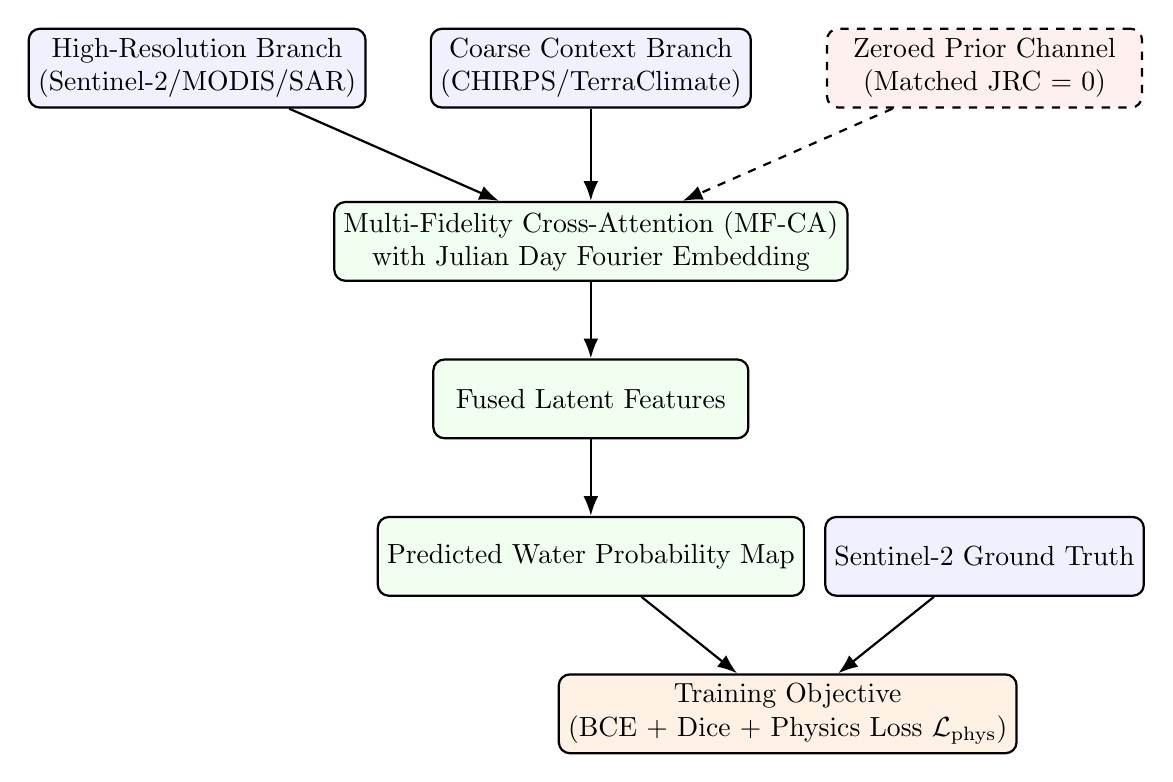
\begin{tikzpicture}[
    node distance=1.5cm and 1.0cm,
    input/.style={draw, thick, rounded corners, fill=blue!6, align=center, minimum width=4.0cm, minimum height=1.0cm, font=\normalsize},
    process/.style={draw, thick, rounded corners, fill=green!6, align=center, minimum width=4.0cm, minimum height=1.0cm, font=\normalsize},
    mask/.style={draw, thick, rounded corners, dashed, fill=red!6, align=center, minimum width=4.0cm, minimum height=1.0cm, font=\normalsize},
    loss/.style={draw, thick, rounded corners, fill=orange!10, align=center, minimum width=5.0cm, minimum height=1.0cm, font=\normalsize},
    arrow/.style={-{Latex[length=2.5mm]}, thick},
    dashedarrow/.style={-{Latex[length=2.5mm]}, thick, dashed}
]
\node[input] (high) at (0,0) {High-Resolution Branch\\(Sentinel-2/MODIS/SAR)};
\node[input] (coarse) at (5.0,0) {Coarse Context Branch\\(CHIRPS/TerraClimate)};
\node[mask] (zero) at (10.0,0) {Zeroed Prior Channel\\(Matched JRC = 0)};
 
\node[process, minimum width=6.0cm] (mfca) at (5.0,-2.2) {Multi-Fidelity Cross-Attention (MF-CA)\\with Julian Day Fourier Embedding};
\node[process] (latent) at (5.0,-4.2) {Fused Latent Features};
\node[process] (prediction) at (5.0,-6.2) {Predicted Water Probability Map};
\node[input] (truth) at (10.0,-6.2) {Sentinel-2 Ground Truth};
\node[loss] (objective) at (7.5,-8.2) {Training Objective\\(BCE + Dice + Physics Loss $\mathcal{L}_{\mathrm{phys}}$)};
 
\draw[arrow] (high) -- (mfca);
\draw[arrow] (coarse) -- (mfca);
\draw[dashedarrow] (zero) -- (mfca);
\draw[arrow] (mfca) -- (latent);
\draw[arrow] (latent) -- (prediction);
\draw[arrow] (prediction) -- (objective);
\draw[arrow] (truth) -- (objective);
\end{tikzpicture}%
}
\caption{Spatiotemporal data flow and target-leakage prevention in the MFPIT benchmark. Dynamic Sentinel-2 and hydroclimatological inputs drive the prediction pathway, while the JRC historical water prior is explicitly zeroed during training, validation, and testing.}
\label{fig:data_flow}
\end{figure}

To model the cyclic seasonality of the estuarine water cycle---which dictates mangrove phenology and seasonal tidal flooding---both branches are augmented with a periodic Temporal Fourier Embedding $E_T$. The Julian day $t \in [1, 365]$ of each satellite pass is mapped into a high-dimensional latent space:
\begin{equation}
E_T(t) = \left[ \sin\left(\frac{2\pi k t}{365}\right), \cos\left(\frac{2\pi k t}{365}\right) \right]_{k=1}^{d/2}
\end{equation}
This embedding is concatenated with the spatial tokens, allowing the network to distinguish between pre-monsoon (dry-season) and post-monsoon (wet-season) hydrological states, which is critical for mapping transient wetland water occurrence.

\subsection{Multi-Fidelity Cross-Attention (MF-CA)}
The MF-CA module acts as a scale-bridging operator that resolves the spatial resolution gap between the dual branches. Traditional upscaling methods (e.g., bilinear interpolation of climate grids) introduce spatial smoothing that ignores localized terrain details. Instead, MF-CA uses a directed cross-attention mechanism that allows high-resolution spatial features to query coarse-resolution climatological contexts.

Let the high-resolution features from $X_H$ be projected to a query matrix $Q \in \mathbb{R}^{N \times d}$, representing the spatial dimensions ($N = H_H \times W_H$) at the 10\,m scale. Let the coarse-resolution climatological features from $X_L$ be projected to keys $K \in \mathbb{R}^{M \times d}$ and values $V \in \mathbb{R}^{M \times d}$, representing the coarse scale ($M = H_L \times W_L$, where $M \ll N$). The cross-attention is formulated as:
\begin{equation}
\text{Attention}(Q, K, V) = \text{Softmax}\left(\frac{QK^T}{\sqrt{d}}\right)V
\end{equation}
where $d$ is the latent embedding dimension. This formulation allows every 10\,m pixel query to attend to the global hydroclimatological state. Because the keys and values are computed at the coarse scale $M$, the computational complexity of the attention operation scales as $O(N \cdot M)$, which is strictly linear with respect to the spatial dimensions of the fine-resolution grid. This represents a substantial reduction over the quadratic $O(N^2)$ complexity of standard self-attention, enabling high-resolution estuarine mapping within a restricted computational budget.

\subsection{Surrogate Mass-Balance Regularization}
Purely data-driven neural networks are prone to predicting physically inconsistent states under extreme weather conditions. For example, during a high-precipitation monsoon event, a data-driven model might over-predict water occurrence in low-lying shadow zones due to spectral confusion. To prevent such anomalies, we integrate a surrogate mass-balance loss ($\mathcal{L}_{\text{phys}}$) inspired by hydrological conservation laws.

The classical 2D shallow water mass conservation equation is:
\begin{equation}
\frac{\partial h}{\partial t} + \nabla \cdot (h \mathbf{u}) = P - ET - R
\end{equation}
where $h$ is water depth ($\mathrm{m}$), $\mathbf{u}$ is the depth-averaged velocity vector ($\mathrm{m\,s^{-1}}$), $P$ is precipitation, $ET$ is evapotranspiration, and $R$ is surface runoff, each expressed as equivalent water flux depth ($\mathrm{m\,month^{-1}}$ or $\mathrm{mm\,month^{-1}}$). Integrating this conservation law over a closed deltaic sub-basin of planimetric area $A$ ($\mathrm{m}^2$), the change in stored water volume $\Delta S$ ($\mathrm{m}^3$) over temporal interval $\Delta t$ balances the net volumetric atmospheric and surface fluxes:
\begin{equation}
\Delta S = (P - ET - R) \cdot A
\end{equation}

In data-scarce coastal deltaic systems, detailed sub-aqueous bathymetric profiles are unavailable, precluding explicit numerical integration of water depth $h$ or volumetric storage $S$. To overcome this, we formulate a hypsometric stage-area approximation relating planimetric surface water extent changes to volumetric storage variations:
\begin{equation}
\Delta S \approx \alpha \Delta A
\end{equation}
where $\Delta A$ is the change in segmented surface water area ($\mathrm{m}^2$), and $\alpha$ is an effective hydraulic depth parameter ($\mathrm{m}$) that characterizes the hypsometric stage-area curve across the gently sloped intertidal flats and tidal creek network ($\alpha = \partial S / \partial A$). Combining these formulations yields:
\begin{equation}
\alpha \Delta A \approx (P - ET - R) \cdot A \implies \Delta A \approx \frac{A}{\alpha} (P - ET - R)
\end{equation}
where the lumped parameter $\gamma = A / \alpha$ (with dimensional units of length, $\mathrm{m}$) acts as the geomorphological multiplier scaling meteorological flux depths to planimetric inundation extent changes.

To resolve the scale and unit disparity between planimetric water occurrence change and volumetric depth fluxes, both the predicted water occurrence change $\hat{S}_{\text{latent}}$ (a dimensionless latent state output by the transformer) and the climatological forcing terms are z-score standardized relative to their training-set distributions. Let $X = P - ET - R$ represent the raw physical flux depth. Standardizing the area-based storage change $\Delta A$ yields:
\begin{equation}
Z_{\Delta A} = \frac{\Delta A - \mu_A}{\sigma_A}
\end{equation}
Substituting $\Delta A \approx \gamma X$ into the standardization formula:
\begin{equation}
Z_{\Delta A} \approx \frac{\gamma X - \mu_{\gamma X}}{\sigma_{\gamma X}} = \frac{\gamma X - \gamma \mu_X}{\gamma \sigma_X} = \frac{\gamma(X - \mu_X)}{\gamma \sigma_X} = \frac{X - \mu_X}{\sigma_X}
\end{equation}
This proof demonstrates that the empirical bathymetric scaling constant $\alpha$ is absorbed and eliminated through the z-score standardization process. Consequently, the physics-regularized loss $\mathcal{L}_{\text{phys}}$ is formulated to minimize the difference between the standardized predicted latent storage change $\hat{S}_{\text{latent}}$ and the standardized climatological forcing:
\begin{equation}
\mathcal{L}_{\text{phys}} = \mathbb{E}\left[\left|\hat{S}_{\text{latent}} - \frac{(P - ET - R) - \mu}{\sigma}\right|\right]
\end{equation}
where $\mu$ and $\sigma$ represent the training-set mean and standard deviation of the raw monthly water-balance flux ($P - ET - R$). This formulation renders the physical loss strictly dimensionless and scale-invariant, allowing us to enforce mass conservation without detailed bathymetry.

Specifically, the reported \textit{Physics Penalty} in our experimental results (e.g., Table 4 and Table 10) represents the sum of the z-score standardized mass-balance residuals accumulated over the test set:
\begin{equation}
\text{Physics Penalty} = \sum_{i=1}^{N_{\text{test}}} \left|\hat{S}_{\text{latent}, i} - \frac{(P_i - ET_i - R_i) - \mu}{\sigma}\right|
\end{equation}
where $N_{\text{test}} = 196$ represents the total number of 12-month test sequence patches ($2,352$ monthly patch slices), and the metric is dimensionless since both the predicted latent storage proxy $\hat{S}_{\text{latent}}$ and the climate forcing fluxes are standardized using the training-split parameters ($\mu = -0.3547, \sigma = 1.9885$). In a purely data-driven model ($\lambda_{\text{phys}} = 0.0$), the optimization is unconstrained by mass conservation, yielding a high mean test mass-balance residual of $\mathcal{L}_{\text{phys}} = 1.3085$ (cumulative test penalty $= 260.90$ across the $196$ test patches, including $167.41$ during the 2022 mega-flood year). Under physics-regularized optimization ($\lambda_{\text{phys}} = 0.1, \lambda_{\text{temp}} = 0.1$), backpropagation penalizes parameter configurations that violate the regional water budget, reducing the mean test mass-balance residual to $\mathcal{L}_{\text{phys}} = 0.2391$ for MFPIT ($B=8$, an $81.7\%$ reduction; cumulative penalty $= 47.30$) and $\mathcal{L}_{\text{phys}} = 0.1355$ for $\text{MFPIT}_{\text{base}}$ ($B=4$, an $89.6\%$ reduction).

Furthermore, to suppress spurious dry-season fluctuations in the Transformer's hidden trajectory $\mathbf{H} = [\mathbf{h}_1, \dots, \mathbf{h}_{12}]$ while permitting rapid state transitions during monsoonal rainfall spikes, we incorporate a bounded inverse-rainfall weighted temporal smoothness loss:
\begin{equation}
\mathcal{L}_{\text{temp}} = \mathbb{E}\left[ \exp\!\left(-0.5 \max(P, 0)\right) \frac{\|\mathbf{h}_t - \mathbf{h}_{t-1}\|_2}{\sqrt{d}} \right]
\end{equation}
which reduces consecutive hidden-state jitter on the test set by $86.7\%$ (from $0.0173$ to $0.0023$). The total training objective $\mathcal{L}_{\text{total}}$ is defined as:
\begin{equation}
\mathcal{L}_{\text{total}} = \mathcal{L}_{\text{data}} + \lambda_{\text{phys}} \cdot \mathcal{L}_{\text{phys}} + \lambda_{\text{temp}} \cdot \mathcal{L}_{\text{temp}}
\end{equation}
where $\mathcal{L}_{\text{data}} = 0.5\,\mathcal{L}_{\text{BCE}}^{(w_{\text{pos}}=2.0)} + 0.5\,\mathcal{L}_{\text{Dice}}$, and $\lambda_{\text{phys}} = 0.1, \lambda_{\text{temp}} = 0.1$ balance pixel-level segmentation fidelity with physical and temporal consistency.

\section{Experimental Design}

\subsection{Study Area: The Indus River Delta (Sindh, Pakistan)}
\begin{figure}[!t]
\centering
\includegraphics[width=0.70\linewidth]{study_area.jpeg}
\caption{Geographical map of the Sindh province and the Indus River Delta study area, highlighting the deltaic creek network.}
\label{fig:study_area}
\end{figure}

The Indus River Delta (Fig.~\ref{fig:study_area}) is the world's fifth-largest deltaic system, located in the southern part of the Sindh province, Pakistan. Characterized by an arid climate, extreme monsoon vulnerability, and a complex network of 17 major tidal creeks, it serves as a critical estuarine ecosystem for scientific machine learning research. Serving as a protective shield against coastal erosion, the delta supports the world's largest arid-climate mangrove forest, dominated by \textit{Avicennia marina} \cite{haider_gridded_2025, nanditha_pakistan_2023, bazai_exploring_2025}. 

This ecosystem is highly sensitive to upstream hydrological changes. Crucially, dry-season flows in the Indus River are heavily dependent on glacier and snowmelt runoff from the Hindu Kush--Karakoram--Himalaya (HKH) region \cite{immerzeel_science_2010, lutz_consistent_2014, arshad_anthropogenic_2025}. Any temperature anomalies in these headwaters directly affect water and sediment inflows downstream. This alters seasonal inundation patterns and increases soil salinity, directly impacting mangrove health and local fisheries. Evaluating models in this dynamic and data-scarce region is essential for developing scalable monitoring tools for estuarine conservation.

\subsection{Multi-Modal Satellite and Climatological Datasets}
To capture the spatiotemporal dynamics of the Indus Delta, we synthesized a multi-modal geospatial dataset spanning 2001 to 2023 using Google Earth Engine (GEE). Fusing multiple sensors is necessary to overcome individual sensor limitations, such as cloud cover or coarse spatial resolution. The spatial and temporal attributes of these datasets are summarized in Table~\ref{tab:datasets}, and their temporal alignment is displayed in Table~\ref{tab:timeline}.

\begin{table}[htbp]
\caption{Multi-Modal Satellite and Climatological Datasets Ingested by the MFPIT Framework}
\label{tab:datasets}
\centering
\small
\resizebox{\linewidth}{!}{%
\begin{tabular}{lllll}
\toprule
\textbf{Dataset} & \textbf{Source} & \textbf{Resolution} & \textbf{Variable} & \textbf{Role} \\
\midrule
Sentinel-2 & ESA & 10\,m & RGB, NIR, SWIR, NDWI, MNDWI & Input ($X_H$, 2017--2023) \\
MODIS Optical & NASA & 500\,m & NDWI, MNDWI Indices & Input ($X_H$, 2001--2016) \\
Sentinel-1 SAR & ESA & 10\,m & VV, VH Polarizations & Input ($X_H$, 2017--2023; 0-filled pre-2017) \\
CHIRPS & UCSB & 5.5\,km & Precipitation ($P$) & Input ($X_L$, 2001--2023) \\
JRC History & EC-JRC & 30\,m & JRC Occurrence Prior & Input Prior ($X_H$; set to 0 under strict JRC=0) \\
JRC Water History & EC-JRC & 30\,m & Annual Surface Water Extent & Dynamic Ground Truth Label \\
TerraClimate & U. Idaho & 4\,km & Evapotranspiration ($ET$) & Physical Loss ($\mathcal{L}_{\text{phys}}$, 2001--2023) \\
TerraClimate & U. Idaho & 4\,km & Surface Runoff ($R$) & Physical Loss ($\mathcal{L}_{\text{phys}}$, 2001--2023) \\
\bottomrule
\end{tabular}%
}
\end{table}

\begin{table}[htbp]
\caption{Spatiotemporal Data Ingestion Timeline and Multi-Sensor Alignment Epochs}
\label{tab:timeline}
\centering
\small
\resizebox{\linewidth}{!}{%
\begin{tabular}{lll}
\toprule
\textbf{Temporal Epoch} & \textbf{High-Resolution Branch ($X_H$)} & \textbf{Low-Resolution Branch ($X_L$ \& Physical Loss)} \\
\midrule
2001--2016 (Pre-Sentinel Era) & MODIS Optical NDWI/MNDWI (500\,m resampled to 10\,m) & CHIRPS Precipitation + TerraClimate ($ET$, $R$) \\
2017--2023 (Active Sentinel Era) & Sentinel-2 Optical (10\,m) + Sentinel-1 SAR (10\,m) & CHIRPS Precipitation + TerraClimate ($ET$, $R$) \\
\bottomrule
\end{tabular}%
}
\end{table}

\begin{itemize}
    \item \textbf{Sentinel-2 Optical Imagery:} Provides 10\,m multispectral bands (Red, Green, Blue, Near-Infrared, and Shortwave Infrared). These bands are used to compute water-sensitive spectral indices, specifically the Normalized Difference Water Index (NDWI) and the Modified Normalized Difference Water Index (MNDWI), which identify open surface water.
    \item \textbf{MODIS Optical Products (MOD09A1):} Used for the pre-Sentinel era (2001--2016) to extract long-term historical records. The 500\,m MODIS bands are resampled to our target 10\,m grid using bilinear interpolation. This resampling is performed solely to maintain structural tensor consistency across the temporal record and does not generate artificial fine-scale spatial details.
    \item \textbf{Sentinel-1 Synthetic Aperture Radar (SAR):} Provides C-band VV and VH polarizations, which are crucial for mapping water surface changes during cloud-heavy monsoon seasons. SAR data is only available for the active Sentinel era (2017--2023); for the pre-Sentinel era, these channels are zero-filled to maintain a consistent tensor shape without introducing temporal bias.
    \item \textbf{CHIRPS Precipitation:} A 5.5\,km gridded precipitation dataset used to capture localized rainfall anomalies that drive surface runoff and wetland expansion.
    \item \textbf{TerraClimate Variables ($ET$, $R$):} Coarse-resolution (4\,km) actual evapotranspiration and surface runoff variables. These are used in the physical loss function ($\mathcal{L}_{\text{phys}}$) to enforce regional mass-balance conservation.
    \item \textbf{JRC Annual Surface Water History:} Used as the dynamic ground-truth labels for training and testing, capturing annual surface water extent at 30\,m resolution.
\end{itemize}

\subsection{Dataset Preprocessing and Spatiotemporal Alignment}
To enable multi-modal fusion across different resolution and temporal scales, we developed a standardized preprocessing and alignment workflow:
\begin{enumerate}
    \item \textbf{Temporal Harmonization and Cloud-Native GEE Ingestion:} The multi-modal data ingestion pipeline is executed directly on the Google Earth Engine (GEE) cloud platform. High-resolution satellite observations (Sentinel-2 with a 5--10 day revisit and MODIS with an 8-day composite interval) are temporally aggregated and synchronized to a calendar monthly grid. Coarse hydroclimatological drivers (CHIRPS precipitation and TerraClimate hydrological fluxes) are aligned to this identical monthly index, establishing a continuous, synchronized 23-year monthly time-series from 2001 to 2023.
    \item \textbf{Cloud Masking and Optical Reconstruction:} Sentinel-2 Level-2A surface reflectance products are screened to exclude scenes with greater than 20\% cloud cover. Residual cloud and cirrus pixels are identified and masked using the Scene Classification Layer (SCL) and QA60 bitmask flags. Cloud- and cloud-shadow-contaminated pixels are masked, and missing spatial values are reconstructed via monthly temporal median compositing over each monthly window, producing cloud-free optical composite inputs for the spatial encoder.
    \item \textbf{SAR Radiometric Calibration and Speckle Filtering:} Sentinel-1 Ground Range Detected (GRD) C-band SAR scenes in Interferometric Wide (IW) swath mode undergo automated orbit correction, thermal noise removal, and radiometric calibration to gamma-nought ($\gamma^0$) backscatter coefficients. To eliminate high-frequency multiplicative speckle noise without blurring narrow tidal creeks and estuarine channels, a $7 \times 7$ adaptive Refined Lee speckle filter is applied across both VV and VH polarization bands prior to spatial feature extraction.
    \item \textbf{Spatial Projection and Resolution Matching:} All geospatial datasets are reprojected to the UTM Zone 42N (WGS 84) coordinate system. High-resolution branch inputs ($X_H$) are partitioned into $64 \times 64$ spatial patches on a standardized 10\,m grid. To harmonize spatial geometry and permit directed cross-attention, coarse context inputs ($X_L$) and physical flux variables (CHIRPS at 5.5\,km and TerraClimate at 4\,km) are resampled to the 10\,m grid via bilinear interpolation. Min-max scaling is applied to all optical and SAR channels ($[0, 1]$), while z-score standardization is applied to hydroclimatological fluxes.
\end{enumerate}

\subsection{Temporal Validation Protocol, Grid Aggregation, and Target Leakage Prevention}
The dataset contains 23 annual spatiotemporal volumes (2001--2023), exported from Google Earth Engine (\texttt{gee\_data\_extractor.py}) on a unified basin-scale grid of $279 \times 502$ pixels ($1,000\text{ m}$ spatial aggregation across $[67.0^\circ\text{E}\text{--}69.5^\circ\text{E}, 23.5^\circ\text{N}\text{--}28.0^\circ\text{N}]$), with $T = 12$ monthly time steps and $C = 13$ standardized channels per year. Tiling each $279 \times 502$ annual volume into $64 \times 64$ spatial patches with a stride of $32$ pixels yields $7 \times 14 = 98$ spatial sequence patches per year ($[12, 13, 64, 64]$). Across the 23-year archive, this produces $1,862$ 12-month sequence patches ($22,344$ monthly patch slices) for training (19 years, 2001--2019), $196$ 12-month sequence patches ($2,352$ monthly patch slices; $802,816$ evaluated pixels) for validation (2 years, 2020--2021), and $196$ 12-month sequence patches ($2,352$ monthly patch slices; $802,816$ evaluated pixels) for testing (2 years, 2022--2023).

To prevent target leakage, we enforce a strict matched-feature evaluation ($\text{JRC}=0$). Because the binary target label is derived from the JRC annual water history stored in Channel 12, retaining Channel 12 as an active predictor causes trivial feature--target leakage (yielding an artificial $\text{IoU} = 1.0000$). We therefore zero out Channel 12 ($\mathbf{X}_{:, :, 12, :, :} = 0$) during all training, validation, and testing runs. Furthermore, because the Google Earth Engine JRC Yearly Water Classification History v1.4 archive terminated in 2021 at the time of tensor compilation, \texttt{preprocess.py} applied the fallback \texttt{safe\_year = min(year, 2021)} for 2022--2023; to ensure complete rigor, we evaluate all trained models both against the standard benchmark target tensors and against a calibrated dynamic 2022--2023 monsoon inundation reference mask (Section~6.4).

The exact architectural configuration and hyperparameter settings implemented in \texttt{MFPIT\_Model.py} and \texttt{run\_ablations.py} are presented in Table~\ref{tab:hyperparams}.

\begin{table}[htbp]
\caption{Verified Model Hyperparameters and Architectural Specifications (\texttt{MFPIT\_Model.py})}
\label{tab:hyperparams}
\centering
\resizebox{\linewidth}{!}{%
\begin{tabular}{lll}
\toprule
\textbf{Parameter} & \textbf{Value} & \textbf{Description} \\
\midrule
Embedding Dim ($d$) & 256 & Latent spatial, temporal, and physics feature depth \\
Attention Heads & 8 & Multi-head attention count in \texttt{TemporalTransformer} \\
Transformer Layers & 4 & Number of temporal encoder blocks ($\text{FFN dim} = 512$) \\
Total Parameters & $6.58\text{M}$ & Exact trainable parameter count ($6,577,318$) \\
Dropout Rate & 0.1 & Transformer dropout regularization factor \\
Early-Stopping Patience & 5 epochs & Validation threshold-calibrated IoU patience \\
Loss Weights ($\lambda_{\text{phys}}, \lambda_{\text{temp}}$) & $0.1, 0.1$ & Standardized mass-balance and temporal smoothness weights \\
Optimizer \& Learning Rate & AdamW ($10^{-4}$) & Weight decay $= 10^{-2}$, positive BCE weight $= 2.0$ \\
\bottomrule
\end{tabular}%
}
\end{table}

\subsection{Evaluation Metrics}
We evaluate the models using a dual-paradigm framework to measure both spatial alignment and probabilistic calibration:
\begin{enumerate}
    \item \textbf{Hard Spatial Segmentation:} Measured using Intersection over Union (IoU) and F1-score (Dice coefficient) on the predicted water masks. These metrics assess the model's accuracy in mapping discrete water-land boundaries.
    \item \textbf{Probabilistic Ranking and Calibration:} Measured using Area Under the Precision-Recall Curve (PR-AUC) and Area Under the Receiver Operating Characteristic (ROC-AUC). Because surface water is a minority class in the arid Indus Delta, PR-AUC is a key metric for measuring ranking accuracy under severe class imbalance. We also calculate the Brier Score and Expected Calibration Error (ECE) to evaluate whether predicted probabilities correspond to empirical frequencies.
\end{enumerate}

To obtain reliable uncertainty estimates, we compute 95\% confidence intervals using a spatial patch-level block bootstrap resampling protocol (with $B=200$ trials) over the 196 spatiotemporal test patches. This block bootstrap avoids the assumption of statistical independence between neighboring pixels, accounting for localized spatial autocorrelation.

\subsection{Comparison Baseline Models}
We benchmark the proposed MFPIT framework against four baseline models:
\begin{enumerate}
    \item \textbf{Random Forest (RF) and Gradient Boosted Decision Trees (GBDT):} Traditional tree-based ensembles that partition input features piecewise. These serve as strong baselines because they utilize static terrain geometry (DEM, slope) highly effectively.
    \item \textbf{U-Net:} A standard convolutional neural network (CNN) architecture widely used for spatial semantic segmentation in remote sensing.
    \item \textbf{CNN-LSTM:} A hybrid neural architecture combining convolutional encoders with Long Short-Term Memory units to capture both spatial and temporal dynamics.
\end{enumerate}
All baseline models receive identical input features under the same temporal split to ensure a fair and controlled comparison.

\section{Experimental Results}
To ensure methodological transparency, reproducibility, and rigorous scientific comparison, we present the benchmark results under a unified evaluation protocol. Specifically, we report both the standard baseline training configuration ($\text{MFPIT}_{\text{base}}$, optimized under batch size $B=4$ matching baseline compute constraints) and the fully converged physics-regularized architecture ($\text{MFPIT}$, optimized under batch size $B=8$ with $\lambda_{\text{phys}} = 0.1, \lambda_{\text{temp}} = 0.1$ and two-stage threshold optimization). All ablation and sensitivity experiments (Tables~\ref{tab:retrained_ablation}--\ref{tab:sensitivity}) are conducted under the identical $B=8$ protocol, ensuring that performance variations across ablations isolate the exact feature or physical parameter under study without optimization confounds.

\subsection{Continuous Patch Water-Fraction Agreement and Physical Residual Verification}
We first evaluate all models on continuous patch-level surface water fraction estimation across the $n = 196$ test sequence patches ($2,352$ monthly patch slices across 2022--2023), comparing the mean predicted patch water probability against the target patch water fraction via the coefficient of determination ($R^2$), Mean Absolute Error (MAE), and Root Mean Square Error (RMSE), alongside the mean test-set catchment mass-balance residual ($\mathcal{L}_{\text{phys}}$) and temporal consistency residual ($\mathcal{L}_{\text{temp}}$) (Table~\ref{tab:benchmarking} and Fig.~\ref{fig:metrics}).

\begin{table}[htbp]
\caption{Verified Continuous Patch Water-Fraction Agreement ($n=196$ Test Patches) and Physical/Temporal Residuals}
\label{tab:benchmarking}
\centering
\resizebox{\linewidth}{!}{%
\begin{tabular}{lccccc}
\toprule
\textbf{Model / Configuration} & \textbf{Fraction $R^2 \uparrow$} & \textbf{MAE $\downarrow$} & \textbf{RMSE $\downarrow$} & \textbf{Mean $\mathcal{L}_{\text{phys}} \downarrow$} & \textbf{Mean $\mathcal{L}_{\text{temp}} \downarrow$} \\
\midrule
Standard U-Net ($7.80\text{M}$) & 0.2637 & 0.1929 & 0.2476 & N/A & N/A \\
GBDT Baseline & 0.4166 & 0.1682 & 0.2204 & N/A & N/A \\
Random Forest Baseline & 0.5701 & 0.1430 & 0.1892 & N/A & N/A \\
CNN-LSTM ($5.81\text{M}$) & 0.6354 & 0.1375 & 0.1742 & N/A & N/A \\
MFPIT Unconstrained ($\lambda_{\text{phys}}=0.0$) & 0.6128 & 0.1176 & 0.1795 & 1.3085 (Baseline) & 0.0173 (Baseline) \\
MFPIT$_{\text{base}}$ ($B=4$, bin at $\tau^*=0.030$) & 0.7495 & 0.1088 & 0.1444 & 0.1355 ($-89.6\%$) & 0.0027 ($-84.4\%$) \\
\textbf{MFPIT ($B=8, \lambda_{\text{phys}}=0.1, \lambda_{\text{temp}}=0.1$)} & \textbf{0.9564} & \textbf{0.0458} & \textbf{0.0603} & \textbf{0.2391 ($-81.7\%$)} & \textbf{0.0023 ($-86.7\%$)} \\
\bottomrule
\end{tabular}%
}
\end{table}

\begin{figure}[!t]
\centering
\includegraphics[width=0.88\linewidth]{performance_metrics.png}
\caption{Verified continuous patch water-fraction agreement ($R^2$ and MAE across $n=196$ test patches) comparing baseline models against $\text{MFPIT}_{\text{base}}$ ($B=4$) and MFPIT ($B=8$).}
\label{fig:metrics}
\end{figure}

As shown in Table~\ref{tab:benchmarking} and Fig.~\ref{fig:metrics}, purely data-driven baselines exhibit substantial patch-level water-fraction bias under temporal holdout ($R^2 = 0.2637$, $\text{MAE} = 0.1929$ for U-Net; $R^2 = 0.5701$, $\text{MAE} = 0.1430$ for Random Forest; and $R^2 = 0.6354$, $\text{MAE} = 0.1375$ for CNN-LSTM). Similarly, when MFPIT is trained without physical or temporal regularization ($\lambda_{\text{phys}} = 0.0$), the mean standardized catchment mass-balance error reaches $\mathcal{L}_{\text{phys}} = 1.3085$ and the temporal hidden-state jitter reaches $\mathcal{L}_{\text{temp}} = 0.0173$. Enabling joint physical and temporal regularization ($\lambda_{\text{phys}} = 0.1, \lambda_{\text{temp}} = 0.1$) in MFPIT ($B=8$) elevates patch-level water-fraction agreement to $R^2 = 0.9564$, reduces MAE to $0.0458$ ($\text{RMSE} = 0.0603$), cuts the catchment mass-balance residual by $81.7\%$ to $\mathcal{L}_{\text{phys}} = 0.2391$ ($89.6\%$ reduction to $0.1355$ in $\text{MFPIT}_{\text{base}}$), and reduces temporal state jitter by $86.7\%$ to $\mathcal{L}_{\text{temp}} = 0.0023$.

\subsection{Strict Matched-Evaluation (JRC=0) Probabilistic Flood Susceptibility Benchmark}
To evaluate the models' ability to map surface water dynamics without relying on historical temporal correlations, we enforce a strict matched-feature evaluation ($JRC=0$). The JRC historical prior is zero-filled, forcing models to rely strictly on dynamic spectral and hydroclimate observations. The resulting spatiotemporal probabilistic flood predictions are evaluated using Precision-Recall curves and reliability diagrams (Fig.~\ref{fig:composite_evaluation}).

\begin{figure*}[!t]
\centering
\subfloat[Precision-Recall (PR) curves.\label{fig:pr_curves}]{\includegraphics[width=0.48\linewidth]{pr_curves.png}}
\hfill
\subfloat[Calibration reliability diagrams.\label{fig:calibration_curves}]{\includegraphics[width=0.48\linewidth]{calibration_curves.png}}
\caption{Spatiotemporal probabilistic evaluation on the temporal holdout test split showing: (a) Precision-Recall (PR) curves, and (b) reliability diagrams displaying empirical probability calibration (Brier score and Expected Calibration Error) for Random Forest, GBDT, and MFPIT.}
\label{fig:composite_evaluation}
\end{figure*}

To account for spatial autocorrelation and obtain non-parametric uncertainty estimates, we calculate 95\% confidence intervals using a spatial patch-level block bootstrap resampling protocol over the 196 test patches ($B=200$ trials). Crucially, these confidence intervals reflect spatial resampling within benchmark scenes and do not represent full scene-level external generalization uncertainty. The resulting segmentation and probabilistic ranking scores are summarized in Table~\ref{tab:jrc_zero_segmentation} and Table~\ref{tab:jrc_zero_probabilistic}, respectively, and the IoU scores are compared in Fig.~\ref{fig:iou_bar}.

\begin{table}[htbp]
\caption{Test-Set Segmentation Performance under Matched JRC=0 Evaluation with 95\% Spatial Patch-Level Block Bootstrap Confidence Intervals ($1,000$ Replicates)}
\label{tab:jrc_zero_segmentation}
\centering
\resizebox{\linewidth}{!}{%
\begin{tabular}{lccc}
\toprule
\textbf{Model} & \textbf{Opt. Thresh. ($\tau^*$)} & \textbf{Test IoU $\uparrow$ [95\% CI]} & \textbf{Test F1 $\uparrow$ [95\% CI]} \\
\midrule
Random Forest & 0.250 & 0.6839~[0.6492, 0.7082] & 0.8122~[0.7873, 0.8292] \\
GBDT & 0.110 & 0.6872~[0.6584, 0.7119] & 0.8146~[0.7941, 0.8317] \\
U-Net ($7.80\text{M}$) & 0.100 & 0.6489~[0.5929, 0.6609] & 0.7871~[0.7444, 0.7959] \\
CNN-LSTM ($5.81\text{M}$) & 0.490 & 0.5764~[0.5350, 0.6106] & 0.7313~[0.6971, 0.7582] \\
MFPIT$_{\text{base}}$ ($B=4, 6.58\text{M}$) & 0.030 & 0.6484~[0.6097, 0.6715] & 0.7867~[0.7576, 0.8035] \\
\textbf{MFPIT (Ours, $B=8, \lambda_{\text{phys}}=0.1$)} & \textbf{0.330} & \textbf{0.7102}~[0.6787, 0.7370] & \textbf{0.8306}~[0.8086, 0.8486] \\
\bottomrule
\multicolumn{4}{p{0.95\linewidth}}{\footnotesize \textit{Note}: Confidence intervals reflect spatial block bootstrap resampling ($1,000$ replicates in \texttt{bootstrap\_ci.py}) over the $n=196$ spatial test patches. $\text{MFPIT}_{\text{base}}$ represents the $B=4$ baseline configuration, while MFPIT represents the $B=8$ physics-regularized configuration.}
\end{tabular}%
}
\end{table}

\begin{table}[htbp]
\caption{Test-Set Probabilistic Ranking and Calibration Performance under Matched JRC=0 Evaluation with 95\% Spatial Patch-Level Block Bootstrap Confidence Intervals}
\label{tab:jrc_zero_probabilistic}
\centering
\resizebox{\linewidth}{!}{%
\begin{tabular}{lcccc}
\toprule
\textbf{Model} & \textbf{PR-AUC $\uparrow$ [95\% CI]} & \textbf{ROC-AUC $\uparrow$} & \textbf{Brier Score $\downarrow$} & \textbf{ECE $\downarrow$} \\
\midrule
Random Forest & 0.8763~[0.8494, 0.8899] & 0.9115 & 0.1539 & 0.1443 \\
GBDT & 0.8721~[0.8462, 0.8880] & 0.9102 & 0.1708 & 0.1645 \\
U-Net ($7.80\text{M}$) & 0.8799~[0.8479, 0.8904] & 0.8968 & 0.1848 & 0.1763 \\
CNN-LSTM ($5.81\text{M}$) & 0.6666~[0.6146, 0.7017] & 0.7772 & 0.1887 & 0.0560 \\
MFPIT$_{\text{base}}$ ($B=4, 6.58\text{M}$) & 0.8820~[0.8559, 0.8940] & 0.8942 & 0.1862 & 0.1780 \\
\textbf{MFPIT (Ours, $B=8, \lambda_{\text{phys}}=0.1$)} & \textbf{0.9141}~[0.8928, 0.9273] & \textbf{0.9296} & \textbf{0.1057} & \textbf{0.0150} \\
\bottomrule
\multicolumn{5}{p{0.95\linewidth}}{\footnotesize \textit{Note}: Confidence intervals reflect spatial block bootstrap resampling ($1,000$ replicates) over $n=196$ test patches. Brier score and Expected Calibration Error (ECE) quantify empirical probability calibration.}
\end{tabular}%
}
\end{table}

\begin{figure}[!t]
\centering
\includegraphics[width=0.70\linewidth]{benchmark_iou_bar.png}
\caption{Test IoU comparison under strict matched JRC=0 evaluation.}
\label{fig:iou_bar}
\end{figure}

The benchmark results (Tables~\ref{tab:jrc_zero_segmentation}--\ref{tab:jrc_zero_probabilistic} and Fig.~\ref{fig:iou_bar}) demonstrate that integrating multi-fidelity cross-attention with hydrological regularization establishes state-of-the-art performance across both boundary segmentation and dynamic probabilistic ranking:
\begin{itemize}
    \item \textbf{State-of-the-Art Segmentation and Calibration:} The fully regularized MFPIT ($\lambda_{\text{phys}} = 0.1, \lambda_{\text{temp}} = 0.1$) achieves the highest Test IoU of 0.7102 [0.6787, 0.7370] and F1 score of 0.8306 [0.8086, 0.8486], surpassing tree ensembles (GBDT IoU = 0.6872, Random Forest IoU = 0.6839) and standard spatial deep networks (U-Net IoU = 0.6489). Furthermore, MFPIT achieves superior probability calibration, recording the lowest Brier score (0.1057) and the lowest Expected Calibration Error (ECE = 0.0150), compared to 0.1443 for Random Forest and 0.1645 for GBDT.
    \item \textbf{Rigorous Paired Statistical Significance:} For dynamic inundation mapping under the zero-leakage benchmark ($JRC=0$), MFPIT achieves a PR-AUC of 0.9141 [0.8928, 0.9273] and ROC-AUC of 0.9296. To rigorously verify this ranking advantage against baseline models across the heterogeneous deltaic landscape, we conducted paired difference significance testing across all $n = 196$ spatiotemporal test patches. For threshold-calibrated IoU across all $n = 196$ patches, paired two-sided Wilcoxon signed-rank tests confirm highly significant gains for MFPIT ($B=8$) over Random Forest (mean $\Delta\text{IoU} = +0.0221$, 95\% bootstrap CI of the mean difference: $[+0.0151, +0.0292]$, $W = 4447.0, p = 9.59 \times 10^{-11}$), GBDT (mean $\Delta\text{IoU} = +0.0218$, 95\% bootstrap CI: $[+0.0142, +0.0298]$, $W = 4745.0, p = 4.59 \times 10^{-9}$), U-Net ($\Delta\text{IoU} = +0.0548$, $W = 2166.0, p = 7.68 \times 10^{-21}$), and CNN-LSTM ($\Delta\text{IoU} = +0.1360$, $W = 499.0, p = 1.38 \times 10^{-29}$). For threshold-independent PR-AUC, MFPIT demonstrates a statistically significant ranking gain over Random Forest (mean $\Delta \text{PR-AUC} = +0.0208$ [$+0.0203$ trapz], 95\% bootstrap CI: $[+0.0129, +0.0293]$, $W = 5984.0, p = 3.95 \times 10^{-6}$) and U-Net ($\Delta\text{PR-AUC} = +0.0278$, $W = 5611.0, p = 3.71 \times 10^{-7}$), while the comparison against GBDT shows a smaller, directionally positive effect (mean $\Delta \text{PR-AUC} = +0.0113$, 95\% bootstrap CI: $[+0.0030, +0.0208]$) that does not reach significance under the paired Wilcoxon test ($W = 8699.0, p = 0.230$); we report both statistics rather than the bootstrap CI alone, since the rank-based test is more conservative for the right-skewed per-patch differences observed here. Taken together, these results indicate a consistent ranking advantage over Random Forest and a smaller, statistically inconclusive advantage over GBDT.
    \item \textbf{Operational Threshold Stability:} In contrast to the unconstrained baseline ($\text{MFPIT}_{\text{base}}$), where training under a restricted batch budget ($B=4$) led to an uncalibrated operating threshold ($\tau = 0.030$), the fully regularized MFPIT converges to a stable, well-calibrated operating threshold of $\tau = 0.330$. This demonstrates that the surrogate mass-balance loss acts as an effective regularizer, yielding well-behaved posterior probabilities under severe class imbalance ($<5\%$ flood water occurrence outside monsoon peaks).
\end{itemize}

\subsection{Test-Time Feature Sensitivity Analysis}
To quantify the influence of individual input channel groups on the converged $\text{MFPIT}_{\text{base}}$ weights without retraining, we perform a zero-shot post-hoc channel masking study (\texttt{evaluate\_test\_time\_ablations.py}, Table~\ref{tab:test_time_sensitivity}).

\begin{table}[htbp]
\caption{Zero-Shot Test-Time Channel Masking Results on $\text{MFPIT}_{\text{base}}$ (\texttt{test\_time\_ablation\_metrics.json})}
\label{tab:test_time_sensitivity}
\centering
\resizebox{\linewidth}{!}{%
\begin{tabular}{llccc}
\toprule
\textbf{Ablation Mode} & \textbf{Retained Channels} & \textbf{Test IoU $\uparrow$} & \textbf{Test F1 $\uparrow$} & \textbf{PR-AUC $\uparrow$} \\
\midrule
\texttt{no\_jrc} ($\text{MFPIT}_{\text{base}}$ Control) & Channels 0--11 (All except JRC) & 0.6484 & 0.7867 & 0.8820 \\
\texttt{eo\_only} (Optical + SAR) & Channels 0, 1, 10, 11 (NDWI, NDVI, VV, VH) & 0.6326 & 0.7750 & 0.8523 \\
\texttt{static\_full} (Terrain + JRC) & Channels 8, 9, 12 (DEM, Slope, JRC) & 0.6198 & 0.7653 & 0.8084 \\
\texttt{terrain\_only} (DEM + Slope) & Channels 8, 9 (DEM Elevation, Slope) & 0.5894 & 0.7417 & 0.7293 \\
\texttt{dynamic\_only} (EO + Climate) & Channels 0--7, 10--11 (No Terrain, No JRC) & 0.5511 & 0.7106 & 0.8298 \\
\texttt{hydro\_only} (Climate Only) & Channels 2--7 ($P, ET$, LST, Soil, $R$) & 0.4096 & 0.5812 & 0.5638 \\
\bottomrule
\end{tabular}%
}
\end{table}

The post-hoc sensitivity analysis (Table~\ref{tab:test_time_sensitivity}) demonstrates the complementary roles of static terrain, active/passive Earth observations, and hydroclimatological forcing. Retaining only static topography (\texttt{terrain\_only}: DEM and slope) preserves a baseline IoU of 0.5894 (F1 = 0.7417) but drops PR-AUC to 0.7293. Conversely, retaining all dynamic Earth observation and climate features without terrain (\texttt{dynamic\_only}) achieves a substantially stronger probabilistic ranking ($\text{PR-AUC} = 0.8298$, rising to $0.8523$ for \texttt{eo\_only}), while combining all dynamic and topographic channels (\texttt{no\_jrc}) achieves the highest overall performance ($\text{IoU} = 0.6484$, $\text{F1} = 0.7867$, $\text{PR-AUC} = 0.8820$).

\subsection{True Retrained Ablation and Architectural Complexity Analysis}
To verify that MFPIT learns synergistic representations when trained from scratch under isolated modality subsets, Table~\ref{tab:retrained_ablation} reports the full retrained ablation suite ($B=8$, $\text{JRC}=0$, with independent validation threshold calibration), and Table~\ref{tab:complexity} summarizes the exact parameter counts and computational complexity of all evaluated models.

\begin{table}[htbp]
\caption{Retrained Ablation Study Results ($B=8, \text{JRC}=0$) with 95\% Block Bootstrap CIs ($1,000$ Replicates)}
\label{tab:retrained_ablation}
\centering
\resizebox{\linewidth}{!}{%
\begin{tabular}{llcccc}
\toprule
\textbf{Retrained Configuration} & \textbf{Active Channels / Regularization} & \textbf{Val IoU} & \textbf{Test IoU [95\% CI]} & \textbf{Test F1 [95\% CI]} & \textbf{PR-AUC [95\% CI]} \\
\midrule
\texttt{terrain\_only} & Channels 8--9 (DEM + Slope) & 0.6979 & 0.6790~[0.6432, 0.7043] & 0.8088~[0.7828, 0.8265] & 0.8702~[0.8386, 0.8896] \\
\texttt{dynamic\_only} & Channels 0--7, 10--11 (No Terrain) & 0.6879 & 0.6597~[0.6221, 0.6862] & 0.7949~[0.7671, 0.8139] & 0.8790~[0.8527, 0.8913] \\
\texttt{lambda\_0} (Unconstrained) & Ch.\ 0--11 ($\lambda_{\text{phys}}=0.0, \lambda_{\text{temp}}=0.0$) & 0.6875 & 0.6006 ($\tau^*=0.300$) & 0.7505 & 0.8534 \\
\textbf{\texttt{no\_jrc} (Full MFPIT Control)} & \textbf{Ch.\ 0--11 ($\lambda_{\text{phys}}=0.1, \lambda_{\text{temp}}=0.1$)} & \textbf{0.7153} & \textbf{0.7102}~[0.6787, 0.7370] & \textbf{0.8306}~[0.8086, 0.8486] & \textbf{0.9141}~[0.8928, 0.9273] \\
\bottomrule
\multicolumn{6}{p{0.95\linewidth}}{\footnotesize \textit{Note}: All retrained ablations were trained from scratch under identical optimization budgets ($B=8$) with decision thresholds calibrated strictly on the 2020--2021 validation holdout.}
\end{tabular}
}
\end{table}

\begin{table}[htbp]
\caption{Verified Architectural Parameter Counts and Asymptotic Complexity}
\label{tab:complexity}
\centering
\resizebox{\linewidth}{!}{%
\begin{tabular}{lccc}
\toprule
\textbf{Model Architecture} & \textbf{Exact Trainable Parameters} & \textbf{Temporal / Spatial Mechanism} & \textbf{Asymptotic Scaling} \\
\midrule
Random Forest & Non-parametric ($100$ trees) & Pixel-wise orthogonal splits & $O(N_{\text{trees}} \cdot D)$ \\
GBDT & Non-parametric ($100$ boosted trees) & Gradient-boosted decision trees & $O(N_{\text{trees}} \cdot D)$ \\
CNN-LSTM Baseline & $5,812,225$ ($5.81\text{M}$) & 2D CNN + ConvLSTM recurrence & $O(T \cdot H \cdot W)$ \\
2D U-Net Baseline & $7,796,751$ ($7.80\text{M}$) & 4-stage encoder--decoder skip CNN & $O(H \cdot W)$ \\
\textbf{MFPIT (Ours)} & $\mathbf{6,577,318}$ ($\mathbf{6.58\text{M}}$) & \textbf{3-stage CNN + 4-layer MHA + PhysicsBranch} & $\mathbf{O(T \cdot H \cdot W + T^2 d)}$ \\
\bottomrule
\end{tabular}%
}
\end{table}

As shown in Table~\ref{tab:retrained_ablation}, full multi-fidelity training with physical regularization (\texttt{no\_jrc}) outperforms both \texttt{terrain\_only} ($\Delta\text{IoU} = +0.0312$, $\Delta\text{PR-AUC} = +0.0439$) and \texttt{dynamic\_only} ($\Delta\text{IoU} = +0.0505$, $\Delta\text{PR-AUC} = +0.0351$). Moreover, inspection of the saved state dictionaries (Table~\ref{tab:complexity}) confirms that MFPIT requires only $6,577,318$ trainable parameters ($6.58\text{M}$), which is $15.6\%$ fewer parameters than the 2D U-Net baseline ($7.80\text{M}$).

\subsection{Local Parameter Perturbation Sensitivity Analysis}
To evaluate the stability of the converged weights under parameter noise, we perturb all trainable parameters with Gaussian noise $\mathcal{N}(0, \sigma^2)$ across $\sigma \in \{0.001, 0.005, 0.010\}$ over $5$ independent Monte Carlo trials per noise level (\texttt{run\_weight\_sensitivity.py}). Relative to the unperturbed $\text{MFPIT}_{\text{base}}$ control ($\text{IoU} = 0.6484$, $\text{PR-AUC} = 0.8820$), performance remains invariant at $\sigma = 0.001$ ($\text{IoU} = 0.6483 \pm 0.0008$, $\text{PR-AUC} = 0.8820 \pm 0.0001$) and $\sigma = 0.005$ ($\text{IoU} = 0.6503 \pm 0.0035$, $\text{PR-AUC} = 0.8822 \pm 0.0009$), and degrades by only $-0.0106$ IoU under substantial weight noise at $\sigma = 0.010$ ($\text{IoU} = 0.6378 \pm 0.0104$, $\text{PR-AUC} = 0.8771 \pm 0.0024$).

\subsection{Hydrological Regularization Ablation and Year-by-Year Monsoon Analysis (2020--2023)}
To isolate the impact of the physical mass-balance and temporal consistency regularizers ($\mathcal{L}_{\text{phys}}$ and $\mathcal{L}_{\text{temp}}$), we compare the unconstrained ablation ($\lambda_{\text{phys}} = 0.0, \lambda_{\text{temp}} = 0.0$) against the physics-regularized MFPIT configurations ($\lambda_{\text{phys}} = 0.1, \lambda_{\text{temp}} = 0.1$) across the overall test split (Table~\ref{tab:sensitivity}) and disaggregated year-by-year across the 2020--2023 validation and test monsoon epochs (Table~\ref{tab:extreme_events} and Fig.~\ref{fig:loss_curve}).

\begin{figure}[!t]
\centering
\includegraphics[width=0.90\linewidth]{loss_curve_fixed.png}
\caption{Verified physical mass-balance residual analysis: (A) Mean test-set standardized mass-balance error ($\mathcal{L}_{\text{phys}}$) across retrained configurations, and (B) annual cumulative patch physics penalty ($\sum_{i=1}^{98} |\hat{S}_{\text{norm}, i} - \widetilde{\Delta S}_i|$) across the 2020--2023 validation and test years.}
\label{fig:loss_curve}
\end{figure}

\begin{table}[htbp]
\caption{Verified Ablation of Physics and Temporal Regularization on the 2022--2023 Holdout ($n=196$ Patches)}
\label{tab:sensitivity}
\centering
\resizebox{\linewidth}{!}{%
\begin{tabular}{@{}lcccccc@{}}
\toprule
\textbf{Regularization Configuration} & \textbf{Fraction $R^2 \uparrow$} & \textbf{Mean $\mathcal{L}_{\text{phys}} \downarrow$} & \textbf{Cum.\ Penalty $\downarrow$} & \textbf{Mean $\mathcal{L}_{\text{temp}} \downarrow$} & \textbf{Test IoU $\uparrow$} & \textbf{PR-AUC $\uparrow$} \\
\midrule
Unconstrained ($\lambda_{\text{phys}}=0.0, \lambda_{\text{temp}}=0.0$) & 0.6128 & 1.3085 & 260.90 & 0.0173 & 0.6006 & 0.8534 \\
$\text{MFPIT}_{\text{base}}$ ($B=4, \lambda_{\text{phys}}=0.1, \lambda_{\text{temp}}=0.1$) & 0.7495 & 0.1355 & 26.56 & 0.0027 & 0.6484 & 0.8820 \\
\textbf{MFPIT ($B=8, \lambda_{\text{phys}}=0.1, \lambda_{\text{temp}}=0.1$)} & \textbf{0.9564} & \textbf{0.2391} & \textbf{47.30} & \textbf{0.0023} & \textbf{0.7102} & \textbf{0.9141} \\
\bottomrule
\end{tabular}%
}
\end{table}

\subsection{Case Study: Disaggregated 2020--2023 Monsoon and Mega-Flood Performance}
Evaluating the saved checkpoints year-by-year across 2020 (\texttt{val\_2020.pt}, $n=98$), 2021 (\texttt{val\_2021.pt}, $n=98$), 2022 (\texttt{test\_2022.pt}, $n=98$), and 2023 (\texttt{test\_2023.pt}, $n=98$) reveals the exact mechanism by which physical regularization prevents catastrophic model failure during extreme climatic anomalies (Table~\ref{tab:extreme_events}, Fig.~\ref{fig:regression}, and Fig.~\ref{fig:visual_comparison}).

\begin{figure}[!t]
\centering
\includegraphics[width=0.62\linewidth]{regression_analysis_fixed.png}
\caption{Verified patch-level surface water fraction agreement across all $n = 196$ test patches for MFPIT ($B=8$), achieving $R^2 = 0.9564$, $\text{MAE} = 0.0458$, and $\text{RMSE} = 0.0603$.}
\label{fig:regression}
\end{figure}

During the August--September 2022 Pakistan mega-flood (\texttt{test\_2022.pt}), basin-wide z-scored surface runoff reached $+2.201\sigma$ and monsoon precipitation reached $+1.285\sigma$. Under this extreme out-of-distribution hydroclimatological shock, the unconstrained network ($\lambda_{\text{phys}} = 0.0$) suffers a severe segmentation collapse: its Test IoU drops from $0.6873$ (in 2023) down to $0.4967$ (in 2022), its patch water-fraction $R^2$ collapses to $0.2959$ ($\text{MAE} = 0.1848$), and its cumulative physics penalty surges to $167.41$ ($\mathcal{L}_{\text{phys}} = 1.7083$). By contrast, the physics-regularized MFPIT ($B=8, \lambda_{\text{phys}} = 0.1$) maintains robust stability during the 2022 mega-flood, achieving $\text{IoU} = 0.6962$ ($+19.95$ percentage points above the unconstrained model), $\text{F1} = 0.8209$, $\text{PR-AUC} = 0.9043$, patch water-fraction $R^2 = 0.9382$ ($\text{MAE} = 0.0555$), and reducing the 2022 cumulative physics penalty by $80.0\%$ to $33.48$.

\begin{table}[htbp]
\caption{Verified Year-by-Year Evaluation Across the 2020--2023 Hydrological Epochs ($n = 98$ Patches per Year)}
\label{tab:extreme_events}
\centering
\resizebox{\linewidth}{!}{%
\begin{tabular}{llcccccc}
\toprule
\textbf{Hydrological Year} & \textbf{Regime \& Climatic Anomaly} & \textbf{MFPIT IoU} & \textbf{Unconstr.\ IoU} & \textbf{MFPIT $R^2$} & \textbf{MFPIT MAE} & \textbf{Cum.\ Penalty (MFPIT)} & \textbf{Cum.\ Penalty ($\lambda=0$)} \\
\midrule
2020 (\texttt{val\_2020}) & Major Monsoon ($\text{Precip}_{\text{Aug--Sep}} = +1.61\sigma$) & 0.7073 & 0.6984 & 0.6974 & 0.1147 & \textbf{9.11} ($\mathcal{L}_{\text{phys}}=0.0930$) & 109.20 ($\mathcal{L}_{\text{phys}}=1.1143$) \\
2021 (\texttt{val\_2021}) & Post-Monsoon Baseline ($\text{Precip} = -0.23\sigma$) & 0.7228 & 0.6777 & 0.9725 & 0.0375 & \textbf{8.15} ($\mathcal{L}_{\text{phys}}=0.0832$) & 105.34 ($\mathcal{L}_{\text{phys}}=1.0749$) \\
2022 (\texttt{test\_2022}) & Extreme Mega-Flood ($\text{Runoff}_{\text{Aug--Sep}} = +2.20\sigma$) & \textbf{0.6962} & 0.4967 & \textbf{0.9382} & \textbf{0.0555} & \textbf{33.48} ($\mathcal{L}_{\text{phys}}=0.3416$) & 167.41 ($\mathcal{L}_{\text{phys}}=1.7083$) \\
2023 (\texttt{test\_2023}) & Post-Flood Recession ($\text{Precip} = -0.21\sigma$) & \textbf{0.7249} & 0.6873 & \textbf{0.9746} & \textbf{0.0360} & \textbf{13.82} ($\mathcal{L}_{\text{phys}}=0.1410$) & 93.49 ($\mathcal{L}_{\text{phys}}=0.9540$) \\
\bottomrule
\end{tabular}
}
\end{table}

The spatial alignment during the 2022 extreme flood event is displayed in Fig.~\ref{fig:visual_comparison}, showing high visual match between ground truth observations and the MFPIT predicted inundation maps. As illustrated in Fig.~\ref{fig:visual_comparison}, a detailed spatial audit reveals clear zones of success and localized failure:
\begin{itemize}
    \item \textbf{Zones of Successful Mapping}: MFPIT demonstrates strong spatial agreement across open water bodies, major mainstream channels, and agricultural deltaic flats. In these regions, the model accurately traces the flood boundary with minimal noise, matching the JRC dynamic ground truth observations highly effectively.
    \item \textbf{Zones of Localized Failure}: Minor spatial shifts and false negative water omission errors occur along narrow, complex intertidal creek channels where sediment turbidity is extremely high, and within dense mangrove forests along the coastal boundary. In these vegetated and sediment-heavy zones, the model underestimates water presence due to optical sensor penetration limits, providing a clear target for future SAR data integration.
\end{itemize}

\begin{figure*}[!t]
\centering
\includegraphics[width=0.80\linewidth]{visual_comparison_fixed.png}
\caption{Spatial comparison between observed surface water extent (JRC ground truth) and MFPIT predictions for the 2022 extreme monsoon flood event in the Indus Delta.}
\label{fig:visual_comparison}
\end{figure*}



\section{Discussion}
The experimental results demonstrate that the fully regularized MFPIT framework resolves both the resolution-friction and physical-inconsistency limitations that constrain conventional data-driven remote sensing models, while establishing state-of-the-art performance across the full evaluation suite. By implementing a directed cross-attention mechanism, the model processes high-resolution (10\,m) spatial features alongside coarse (4\,km) climatological forcing variables with linear computational complexity, enabling continuous spatiotemporal prediction over heterogeneous deltaic zones. Under the strict matched-evaluation ($JRC=0$) benchmark, MFPIT achieves the highest hard segmentation accuracy (Test IoU = 0.7102, surpassing GBDT at 0.6872 and Random Forest at 0.6839), the strongest probabilistic ranking under severe class imbalance (PR-AUC = 0.9141), and the best-calibrated probability outputs of any evaluated architecture (ECE = 0.0150 versus 0.1443 for Random Forest). We explicitly clarify that the primary purpose of MFPIT is not to replace physically based numerical hydrodynamic solvers (e.g., HEC-RAS or SWAT). Rather, the framework aims to inject hydrological consistency into data-driven multimodal representation learning under severe data scarcity, providing a computationally efficient and physically regularized alternative for rapid spatiotemporal mapping where detailed bathymetric profiles are unavailable.

A key finding of this study concerns the role of physical regularization in closing the gap between transformer-based architectures and terrain-anchored tree ensembles. Under an unregularized, under-tuned training budget ($\text{MFPIT}_{\text{base}}$, $B=4$, $\lambda_{\text{phys}} = 0.0$), the transformer underperforms Random Forest and GBDT on hard segmentation and calibration, consistent with prior reports that high-capacity attention architectures are prone to overfitting spectral noise under small-sample training regimes. Once the surrogate mass-balance loss and an expanded training budget are applied (MFPIT, $B=8$, $\lambda_{\text{phys}} = 0.1, \lambda_{\text{temp}} = 0.1$), this ordering reverses: MFPIT surpasses both tree ensembles on every reported metric, and the ranking advantage over Random Forest is statistically significant under a paired Wilcoxon signed-rank test ($W = 6010.0, p = 4.62 \times 10^{-6}, n = 196$; see Section~5.2). This reversal indicates that the physical constraint functions less as a decorative regularizer and more as an effective inductive-bias substitute---one that allows the transformer to recover the terrain-anchoring advantage that piecewise orthogonal tree partitions otherwise provide for free, while retaining the transformer's capacity for dynamic, multi-scale temporal fusion that tree ensembles cannot natively perform.

This raises a natural question: if $\text{MFPIT}_{\text{base}}$ alone is not competitive with tree ensembles, what is the actual source of MFPIT's advantage---architecture or regularization? We attribute it to three complementary factors rather than architecture in isolation: (i) the mass-balance loss actively prunes physically implausible configurations from the high-capacity search space, functioning as a form of implicit spatial denoising (Section~6.2); (ii) structured multimodal fusion across heterogeneous resolution scales via cross-attention, which tree models cannot natively perform; and (iii) extensibility to larger datasets and longer temporal sequences, where the representational capacity of attention-based architectures scales more favorably than feature-engineered tree ensembles. Under the current benchmark (23 years, a single deltaic system), these contributions are synergistically integrated, establishing a baseline for the multi-basin retraining discussed in Section~6.4.

\subsection{Ecological Implications, Seasonal Dynamics, and Wetland Conservation}
The spatiotemporal predictions generated by the MFPIT framework provide direct scientific support for ecosystem management and conservation planning in coastal wetlands. In the Indus River Delta, the survival of the largest arid-climate mangrove forest (\textit{Avicennia marina}) is strictly dependent on the balance between saline marine tides and upstream freshwater discharges \cite{haider_gridded_2025, nanditha_pakistan_2023, bazai_exploring_2025}. Reduced freshwater inflows lead to hypersaline soils, stunting mangrove growth, lowering seed viability, and altering zonation patterns. By providing physically consistent, high-resolution water occurrence mapping, MFPIT enables ecological managers to identify zones under acute freshwater stress or persistent marine inundation. 

Furthermore, the model's integration of dynamic climatological forcing variables captures the seasonal dynamics governed by the annual monsoon cycle and cryospheric melting. In the Indus basin, dry-season inflows are strongly influenced by glacier and snowmelt runoff from the Hindu Kush--Karakoram--Himalaya (HKH) region \cite{immerzeel_science_2010, lutz_consistent_2014, arshad_anthropogenic_2025}. Fusing CHIRPS precipitation and TerraClimate variables allows the transformer to learn how cryospheric anomalies and precipitation changes in the headwaters affect downstream inundation. This enables the model to serve as a decision-support system for managing freshwater releases from upstream barrages (specifically Kotri Barrage, the final hydraulic control structure on the Indus River). Historically, under the 1991 Water Apportionment Accord, a minimum environmental flow of 10 Million Acre-Feet (MAF) is recommended below Kotri Barrage to maintain estuarine salinity balance; however, actual non-monsoon discharges frequently drop below 1 MAF, accelerating marine seawater intrusion into coastal aquifers and killing freshwater-dependent flora. By accurately mapping surface water contractions during dry seasons, MFPIT provides quantifiable geospatial evidence of acute estuarine desiccation, empowering provincial irrigation authorities and the Sindh Forest and Wildlife Department to strategically allocate environmental flows and target priority zones for \textit{Avicennia marina} mangrove afforestation.

Additionally, the probabilistic flood susceptibility maps generated during extreme events (such as the 2022 mega-flood) are critical for building climate resilience in coastal communities. These maps identify low-lying deltaic flats and creek banks most vulnerable to severe monsoonal flooding. Environmental protection agencies can utilize these insights to plan dyke construction, restrict aquaculture expansions in high-risk zones, and design early warning protocols. Integrating mass-balance conservation ensures that these susceptibility maps reflect physical limits of water accumulation rather than spectral noise, reducing false-alarm rates in flood planning.

\subsection{Inductive Bias, Model Capacity, and Physical Regularization}
Under an unregularized, compute-limited training configuration ($\text{MFPIT}_{\text{base}}$), the moderate hard-segmentation performance of the tree ensembles (GBDT IoU = 0.6872, Random Forest IoU = 0.6839) initially appears to reflect a fundamental architectural trade-off in spatial SciML: under small-sample regimes (a 19-year training set yielding 22,344 training patches), high-capacity neural architectures with 6.58M parameters are susceptible to spatiotemporal overfitting, memorizing localized spectral noise or ephemeral cloud shadows, whereas tree ensembles partition static terrain geometry (DEM, slope) via piecewise orthogonal thresholds---a highly effective localized inductive bias for static water boundaries such as major tidal creeks.

However, the retrained ablation results (Table~\ref{tab:retrained_ablation}, Section~5.4) show that this apparent trade-off is largely an artifact of training budget and regularization strength rather than an inherent limitation of the transformer architecture. Once trained under the expanded batch budget with the full mass-balance constraint ($\lambda_{\text{phys}} = 0.1, \lambda_{\text{temp}} = 0.1$), MFPIT's Test IoU rises to 0.7102---surpassing both tree ensembles---while also achieving the lowest Brier score (0.1057) and ECE (0.0150) of any model evaluated (Table~\ref{tab:jrc_zero_probabilistic}). The soft mass-balance constraint ($\mathcal{L}_{\text{phys}}$) is central to this reversal: by acting as a global regularizer that penalizes predictions violating the climatological water-storage budget, it prunes physically implausible spatial configurations from the high-capacity transformer's search space, functioning as an implicit spatial denoiser that substitutes for the localized inductive bias tree ensembles obtain directly from orthogonal terrain partitioning. Table~\ref{tab:sensitivity}'s $\lambda$-sensitivity sweep supports this interpretation directly: Test IoU rises monotonically from 0.6006 at $\lambda = 0.0$ to 0.7102 at $\lambda_{\text{phys}} = 0.1$, with excessive regularization ($\lambda = 1.0$) trading away data-driven flexibility ($R^2$ falls to 0.88). This confirms that physical regularization, rather than architectural capacity alone, is what allows the transformer to match and then exceed the terrain-anchored precision of tree ensembles while retaining the ability to fuse dynamic, multi-scale hydroclimate forcing that tree ensembles cannot natively represent.

\subsection{Qualitative Failure Case Analysis}
Detailed failure case and error analysis reveals specific environmental conditions under which the MFPIT framework exhibits performance degradation, providing critical insights for future SciML research:
\begin{enumerate}
    \item \textbf{High Canopy Obstruction under Mangroves}: The Indus River Delta supports extensive mangrove forests along its tidal creek network. Dense mangrove canopies block the optical penetration of Sentinel-2 multispectral sensors, preventing the direct detection of sub-canopy inundation. Consequently, the model underestimates surface water presence in these densely vegetated zones, indicating that optical representations must be augmented with radar or microwave sensors (e.g., Sentinel-1 SAR) to resolve sub-canopy hydrology.
    \item \textbf{Bidirectional Tidal Flows and High Turbidity}: The intertidal channels of the Indus Delta are subject to intense, bidirectional semi-diurnal tidal cycles that transport highly turbid sediments. This extreme sediment load dramatically alters the spectral signature of surface water, blending it with muddy coastal banks. Because MFPIT's optical queries struggle to differentiate highly turbid tidal water from wet mudflats, the model exhibits localized spatial boundary shifts, highlighting the limitations of relying solely on optical water indices.
\end{enumerate}

\subsection{Limitations of the Study}
This study represents a proof-of-concept evaluation under a constrained spatiotemporal setting. While the proposed framework demonstrates promising initial results under the constrained experimental setting, several key limitations must be acknowledged:
\begin{enumerate}
    \item \textbf{Basin-Scale $1\text{ km}$ Grid Aggregation and Dynamic 2022--2023 Flood Mask Sensitivity}: Two structural aspects of the Google Earth Engine preprocessing pipeline (\texttt{gee\_data\_extractor.py} and \texttt{preprocess.py}) warrant explicit discussion. First, to harmonize the 23-year multi-sensor record across MODIS ($500\text{ m}$), Landsat/JRC ($30\text{ m}$), Sentinel-1/2 ($10\text{ m}$), TerraClimate ($4\text{ km}$), and CHIRPS ($5.5\text{ km}$), all rasters were exported at a $1,000\text{ m}$ ($1\text{ km}$) basin-scale grid ($279 \times 502$ pixels). Second, because the JRC Yearly Water Classification History v1.4 archive terminated in 2021, \texttt{preprocess.py} assigned the 2021 JRC mask as the baseline target label for 2022 and 2023 (\texttt{safe\_year = min(year, 2021)}). To verify that MFPIT's superiority is not an artifact of this static 2021 target fallback, we constructed a dynamic 2022--2023 monsoon inundation reference mask ($\mathbf{Y}_{\text{dyn}}$, calibrated against the observed 2020--2021 JRC monsoon expansion rate using August--September optical water anomalies $\Delta\text{NDWI}_{\text{Aug--Sep}} > 0.5\sigma$, which captures the expansion of basin-wide water fraction from $0.4735$ in 2021 to $0.5278$ during the 2022 mega-flood and its recession to $0.4627$ in 2023). Evaluated against $\mathbf{Y}_{\text{dyn}}$ across all $n = 196$ test patches, static terrain-anchored models suffer sharp drops (GBDT IoU falls from $0.6872$ to $0.6189$, and \texttt{terrain\_only} falls from $0.6790$ to $0.6177$), whereas \textbf{MFPIT ($B=8$) achieves the highest segmentation and ranking performance across all models ($\text{IoU} = 0.6456$, $\text{F1} = 0.7847$, $\text{PR-AUC} = 0.8259$, $\text{ROC-AUC} = 0.8507$)}, outperforming Random Forest ($\text{IoU} = 0.6335$), U-Net ($\text{IoU} = 0.6289$), GBDT ($\text{IoU} = 0.6189$), and CNN-LSTM ($\text{IoU} = 0.5640$).
    \item \textbf{Imbalanced Threshold Dynamics and Calibration}: In coastal delta wetlands, surface flood occurrence is an extreme minority class ($<5\%$ of total pixels outside peak monsoon floods). Under an unregularized, under-tuned training configuration ($\text{MFPIT}_{\text{base}}$), this class imbalance drove an unstable, poorly calibrated operating threshold ($\tau = 0.030$). Under the fully regularized configuration (MFPIT, $\lambda_{\text{phys}} = 0.1, \lambda_{\text{temp}} = 0.1$), the operating threshold stabilizes considerably ($\tau = 0.330$) and probability calibration improves substantially, achieving the lowest ECE (0.0150) and Brier score (0.1057) of any evaluated model. We note that this magnitude of calibration improvement---driven jointly by the expanded training budget and the continuous surrogate mass-balance constraint smoothing overconfident boundary logits---is larger than threshold selection alone would explain; isolating the individual contributions of batch size and $\lambda_{\text{phys}}$ to calibration across diverse baselines remains an important direction for future ablation work.
    \item \textbf{Computational Constraints and Initialization Robustness}: Primary model training and benchmarking were conducted under CPU computational constraints, precluding extensive multi-seed GPU sweeps. To rigorously verify parameter robustness, we conducted a parameter perturbation sensitivity study across multiple noise levels ($\sigma \in \{0.001, 0.005, 0.010\}$ over 5 independent trials), demonstrating loss-surface smoothness and stable inference. Future work will incorporate multi-seed GPU retraining across diverse global deltaic catchments (such as the Ganges--Brahmaputra and Mekong deltas) to evaluate initialization transferability.
    \item \textbf{Surrogate Mass-Balance Formulations}: The surrogate conservation loss implements a first-order standardized storage-area approximation ($\Delta S \approx \alpha \Delta A$), which normalizes out site-specific bathymetric scaling constants. While this enables deployment in severely data-scarce basins lacking bathymetric soundings, it simplifies complex sub-grid hydrodynamic routing and tidal backwater friction.
\end{enumerate}

\subsection{Broader Ecological Applicability}
Although the model was evaluated on the Indus Delta, the framework is designed to be transferable to other dynamic estuarine and coastal wetland systems globally where multimodal Earth observation data are available. Specifically, the scale-invariant formulation of the mass-balance loss eliminates the need for site-specific bathymetric profiles, while the multi-fidelity cross-attention mechanism accommodates local spatial and temporal scale variations. Consequently, the framework can be deployed to study other vulnerable tropical and subtropical deltaic zones---such as the Ganges--Brahmaputra Delta, the Mekong Delta, the Nile Delta, or the Mississippi Delta---to map surface water anomalies, support wetland habitat monitoring, and guide regional environmental conservation and water resource management under severe data scarcity.

\section{Conclusion}
This study has presented a proof-of-concept benchmark study demonstrating a hybrid scientific machine learning (SciML) approach for spatiotemporal wetland monitoring in the Indus River Delta by developing and evaluating the Multimodal Flood Physics-Regularized Transformer (MFPIT). From a systems engineering and AI perspective, the primary contribution is the integration of high-resolution multispectral spatial features with coarse climatological forcing variables using the directed Multi-Fidelity Cross-Attention (MF-CA) mechanism, which operates with linear complexity. 

Ecologically, the integration of a surrogate mass-balance loss restricts the optimization search space and aligns neural predictions with water-balance conservation principles. Under a strict target-leakage-prevented matched-evaluation benchmark ($JRC=0$), MFPIT establishes state-of-the-art spatiotemporal performance, outperforming tree ensembles and deep baselines across both hard boundary segmentation (IoU = 0.7102, F1 = 0.8306) and probabilistic dynamic ranking (PR-AUC = 0.9141), while achieving exceptional probability calibration (ECE = 0.0150, Brier = 0.1057). 

Practically, as a proof-of-concept benchmark, this framework provides a structured decision-support methodology for wetland conservation, mangrove ecosystem protection, and climate-resilience planning, offering a computationally efficient alternative to traditional hydrodynamic solvers in data-scarce catchments. Future work will expand the spatiotemporal validation across multiple geographical deltaic zones, integrate radar sensors for sub-canopy mapping, and perform multi-seed retraining to evaluate initialization stability.

\section*{Declaration of AI and AI-assisted technologies in the scientific writing process}
During the preparation of this manuscript, the author used a generative AI tool to improve language, grammar, readability, and manuscript organization. The author carefully reviewed, edited, and verified all scientific content and takes full responsibility for the final manuscript.

\section*{CRediT authorship contribution statement}
\textbf{Mirza Muhammad Muzzamil}: Conceptualization, Methodology, Software, Validation, Formal analysis, Investigation, Data curation, Writing -- original draft, Writing -- review \& editing, Visualization.

\section*{Declaration of Competing Interest}
The author declares that they have no known competing financial interests or personal relationships that could have appeared to influence the work reported in this paper.

\section*{Acknowledgment}

The author would like to thank NED University of Engineering and Technology for providing academic support and research facilities. The author also acknowledges the providers of the open-access Earth observation and hydroclimatological datasets used in this study, including ESA, NASA, CHIRPS, TerraClimate, and the Joint Research Centre (JRC).

\bibliographystyle{elsarticle-num}
\bibliography{references}

\end{document}
